\section{Anforderungsanalyse}
\label{sec:requirements}

Dieses Kapitel beschreibt die generellen Anforderungen an die Entwicklungsumgebung. Dabei werden auch einige theoretische Hintergründe betrachtet, speziell mögliche Reduktionen des SQL-Sprachumfangs für die Vermittlung von Datenbankkenntnissen. Ebenfalls thematisiert werden unterschiedliche Vorgehensweisen um Schüler bei der Entwicklung von Oberflächen sinnvoll anzuleiten. Den Schwerpunkt bildet die Beschreibung der beiden wichtigsten Komponenten der Entwicklungsumgebung: Die spezialisierten Editoren für SQL und Oberflächen.

\warning[Hinweis]{Der Verzicht auf die technischen Hintergründe der Implementierung soll dieses Kapitel auch für Informatik-Interessierte ohne softwaretechnischen Hintergrund verständlich halten, anstatt Sie gleich mit den Details der Realisierung zu erschlagen. Die Planung konkreter Umsetzungsstrategien, inklusive einer Erläuterung von softwaretechnischen Details und verfügbaren Schnittstellen, werden in Kapitel \ref{sec:implementation-analysis}~\nameref{sec:implementation-analysis} besprochen.}

\idename{} geht im Vergleich zu Scratch und dem App Inventor in Bezug auf die gelehrten Programmiersprachen einen anderen Weg: Es lehrt unmittelbar den Umgang mit \texttt{SQL} und \texttt{HTML}, allerdings in gegebenenfalls reduzierten Umfängen (siehe \ref{sec:sql-subset} \nameref{sec:sql-subset} und \ref{sec:design-ui-concept} \nameref{sec:design-ui-concept}). Die Entwicklung eigener Programmier- oder Auszeichnungssprachen für die Lehre mag zwar aus didaktischer Sicht einige Vorteile bieten, geht im Rahmen dieser Arbeit aber auch mit zwei gravierenden Nachteilen einher: Zum Einen ist die Entwicklung einer konsistenten Programmiersprache alles andere als trivial (von Zweien ganz zu schweigen). Zum Anderen erschwert eine solche Insellösung den Übergang zu "`richtiger"' Programmierung in der "`echten"' Welt außerhalb dieser Lehrumgebung. Abgesehen davon handelt es sich bei \texttt{SQL} und \texttt{HTML} um vergleichsweise einfache Sprachen, die sich darüber hinaus gut im Umfang reduzieren lassen. Aus diesen Gründen setzt \idename{} auf bestehende und etablierte Standards auf.

Die in diesem Kapitel "`erträumte"' Konzeption wird aufgrund der Endlichkeit der im Rahmen einer Master-Thesis zur Verfügung stehenden Zeitspanne nicht vollständig umgesetzt werden können. Trotzdem ist eine möglichst vollständige Erfassung von Anforderungen unerläßlich, um im Falle einer Fortführung der Entwicklung nicht aufgrund von unberücksichtigten Anforderungen große Umbauarbeiten vornehmen zu müssen.

Da der Zweck dieser Arbeit die Konzeption und Umsetzung einer Software ist, deren Zweck wiederum die Entwicklung anderer Software ist, bedarf es zunächst eines einheitlichen Verständnisses für die Bezeichnungen der beteiligten Personen und Entitäten:

\begin{description}
\item[(Schüler-)Entwicklungsumgebung, \idename{}] \hfill\\
  Bezeichnet die von den Lernenden zu nutzende Software, die im Rahmen dieser Arbeit erstellt wird. Sofern Verwechslungen mit anderen Entwicklungsumgebungen (engl. ``integrated development environment'', IDE) auftreten könnten, wird explizit das Präfix ``Schüler'' genutzt. Diese Unterscheidung wird insbesondere bei Vergleichen mit gängiger Entwicklungssoftware Art relevant sein.
\item[(Schüler-)Projekt] \hfill\\
  Bezeichnet die von den Lernenden unter Nutzung der Schülerentwicklungsumgebung erstellte Software. Teil eines solchen Projektes sind unter anderem das Datenbankschema, die verschiedenen Abfragen und die gestaltete Benutzeroberfläche.
\item[Entwickler] \hfill\\
  Bezeichnet Personen, die mit der ``entwickelnden'' Benutzeroberfläche eines Schülerprojekts interagieren.
\item[Endanwender] \hfill\\
  Bezeichnet Personen, die mit der von den Entwicklern erstellten ``normalen'' Benutzeroberfläche eines Schülerprojekts interagieren, nicht jedoch mit der Schülerentwicklungsumgebung selbst.
\end{description}

\subsection{Zielgruppe}
\label{sec:target-audience}

Mit \idename{} sollen Schülerinnen und Schüler ab der Mittelstufe angesprochen werden. Die im folgenden genannten Aspekte bilden ein sehr oberflächliches Profil hilfreicher Vorkenntnisse, an denen man sich als Lehrkraft für die Fragestellung "`Sind meine Schüler bereit für \idename{}?"' orientieren könnte. Dieses Profil ist dabei allerdings nicht als striktes Anforderungsprofil zu verstehen: Grundsätzlich lassen sich diese Kenntnisse auch am Beispiel von \idename{} vermitteln. Erfahrungen mit Datenbanken oder Webentwicklung sind hingegen nicht Bestandteil dieses Profils, schließlich versteht sich \idename{} als eine Lernumgebung für genau diese Technologien.

\begin{description}
\item[Grundlegende PC-Anwenderkenntnisse] \hfill\\
  Die Schüler müssen in der Lage sein einen Browser zu bedienen und mit Begriffen wie "`Speichern"' und "`Klicken und Ziehen"' vertraut sein. Kenntnisse des Dateisystems sind jedoch nicht notwendig, \idename{} abstrahiert die konkreten Speicherorte weg.
\item[Tabellenkalkulation] \hfill\\
  Kenntnisse über den Umgang mit Tabellenkalkulationsprogrammen sind keine zwingende Voraussetzung, aber eine sinnvolle Vorstufe um die Strukturierungsmöglichkeiten von Datenbeständen zu verstehen. Sofern sich die Schüler innerhalb eines solchen Programms auch schon mit Funktionen wie \texttt{SUMME} beschäftigt haben, kann auf diesem Wissen aufgebaut werden.
\item[Bedienelemente] \hfill\\
  Wenn die Schüler mit \idename{} eigene Oberflächen entwickeln sollen, brauchen sie grundlegende Vorstellungen über die Funktionsweise und Parameter einiger Bedienelemente: Mit Links werden Inhalte verknüpft, Knöpfe lösen Aktionen aus, Textfelder stellen Werte zur Verfügung, eine Combobox erlaubt die Auswahl von einem Wert aus vielen Werten ... Ohne zu wissen wozu bestimmte Bedienelemte eingesetzt werden, erschließt sich deren Verwendung in \texttt{HTML} nur sehr umständlich.
\item[Englische Vokabeln] \hfill\\
  In der initialen Version wird \idename{} die Syntax von \texttt{SQL} oder \texttt{HTML} zwar vereinfachen und augmentieren, aber nicht übersetzen. Den Schülern sollte die Bedeutung von Fragmenten wie \texttt{WHERE} oder \texttt{<input>} also geläufig sein.
\end{description}

\subsection{Grundprinzipien}
\label{sec:principles}

Nach der Betrachtung der zu bedienenden Zielgruppe und der Beschäftigung mit bereits existierenden Alternativen, ist es zunächst sinnvoll ein paar allgemeine Grundprinzipien zu formulieren. Diese Prinzipien bilden die Philosophie hinter der Schülerentwicklungsumgebung ab und dienen als Leitfaden für Designentscheidungen. Praktisch erlaubt das vor allem eine relativ akkurate Abschätzung, ob sich die Implementierung einer bestimmten Idee lohnt und wie sie zu priorisieren ist. Diese Sortierung dieser Prinzipien ist entsprechend ihrer Bedeutung absteigend sortiert, das wichtigste Prinzip wird also zuerst genannt.

\begin{description}
\item[Semantik vor Syntax] \hfill\\
  Den Lernenden sollen kontextsensitiv sinnvolle Operationen angeboten werden, optimalerweise mit einer kurzen Erläuterung, warum gerade nur diese Teilmenge an Operationen möglich ist. Die eigentliche Programmierung erfolgt dann durch die Kombination von Bausteinen, ähnlich wie bei der Lernsoftware ``Scratch''. Durch kontinuirliches Feedback der Entwicklungsumgebung sollen die Lernenden in die Lage versetzt werden, auch ohne ständige Rückversicherung bei der Lehrkraft eigene Ansätze zu erproben. Syntaxfehler, ein typisches Problem für viele Anfänger, werden durch dieses Vorgehen konstruktiv verhindert.
\item[Motivation durch praktisch vorzeigbare Ergebnisse] \hfill\\
  Der Einstieg in die Programmierung ist oftmals von relativ langweiligen Programmen geprägt, häufig textbasierten Konsolenanwendungen, welche sich nicht gut im Freundes- oder Bekanntenkreis präsentieren lassen. Im Sonderfall der Vermittlung von \texttt{SQL}-Kenntnissen ist das Ergebnis der investierten Arbeit sogar überhaupt nicht sinnvoll zu demonstrieren. Die erstellten Abfragen stehen isoliert für sich und sind häufig auch nur in der Entwicklungsumgebung der jeweiligen Datenbank ausführbar. Mit der im Rahmen dieser Arbeit zu erstellenden Software sollen sich hingegen praktisch relevante, allerdings sehr datenorientierte Programme umsetzen lassen. Diese verfügen über von den Lernenden zusammengestellte Eingabemasken um Daten einzufügen oder zu manipulieren und verschiedene Ausgabesichten um den Datenbestand sinnvoll zu präsentieren.
\item[Schrittweise komplexere Benutzeroberfläche der Entwicklungsumgebung] \hfill \\
  Konventionelle Entwicklungsumgebungen sind Programme von Profis für Profis und bieten einen dementsprechend ausgerichteten Funktionsumfang. Gerade wenn man aber dabei ist etwas Neues zu lernen, kann es sinnvoll sein, die Menge der möglichen Optionen zu beschränken. In diesem Sinne sollte die Lehrkraft die Möglichkeit haben, den Funktionsumfang der Entwicklungsumgebung für Schüler gezielt zu reduzieren. Es sollten sich also Funktionen der Entwicklungsumgebung ausblenden lassen, wenn dies aus didaktischen Gründen sinnvoll erscheint. Zum Beispiel könnten bestimmte Bedienelemente oder Bestandteile von \texttt{SQL} ausgeblendet werden, wenn diese noch nicht behandelt worden sind.
\item[Einfache Inbetriebnahme] \hfill \\
  Eine initiale Hürde jeder (Lern-)Software ist deren Installation, insbesondere bei Programmen aus dem Datenbankumfeld. Die Inbetriebnahme der für Server konzipierten Programme auf privaten, ``normalen'' Rechnern führt immer wieder zu Problemen aufgrund von unerfüllten Abhängigkeiten, fehlenden Rechten beim Starten von Systemdiensten oder bei Dateizugriffen. Die zunehmende Heterogenität an Betriebssystemen, insbesondere die zunehmende Verwendung MacOS \cite{statista-os-verbreitung}, tut ein Übriges um die Verteilung von Software zu erschweren. Damit der eigentliche Lernprozess nicht schon vor dem Start der Entwicklungsumgebung behindert wird, ist eine möglichst einfache Inbetriebnahme von entsprechender Bedeutung. Die Informatiklehrkräfte stehen bei dem Betrieb der jeweiligen Programme in der Schule vor ähnlichen Problemen wie ihre Schüler, nur dass Sie auf die Konfiguration des Rechnerpools ihrer Schule oftmals nur einen eingeschränkten Einfluss haben. Die im Vergleich zu privaten Rechnern wesentlich restriktiver gehandhabte Rechte eines Schul-PCs verkomplizieren dieses Szenario zusätzlich. Damit der Lernprozess mit \idename{} nicht schon mit einer fehlgeschlagenen Installation endet, soll der initiale Kontakt so wenig Hürden wie möglich aufstellen.
\item[Fortführung der entwickelten Projekte] \hfill \\
  Lernumgebungen wie Scratch oder der AppInventor sind in sich geschlossene Systeme, deren Arbeitsergebnisse nur schwer in anderen Programmen oder Kontexten von Nutzen sind. Sobald der Lernende dann die Grenzen der verwendeten Lernsoftware erreicht hat, steckt er in einem Dilemma: Es ist für ihn notwendig auf eine andere Software auszuweichen, in diese kann er sein bestehendes Projekt aber nicht einfach mitnehmen. Die Arbeitsergebnisse dieser zu entwickelnden Software sollen daher zumindest einfach einsehbar sein, optimalerweise nach einem Export sogar mit gängigen Entwicklungsumgebungen oder Texteditoren erweiterbar.
\end{description}

\subsection{Künftigen Erweiterungen vorbehalten}
\label{sec:out-of-scope}

Umgekehrt ist es auch wichtig, den Umfang des zu entwickelnden Programms auf einem im Rahmen der Thesis machbaren Umfang zu begrenzen. Die folgenden Ideen wären mehr oder minder naheliegende Ergänzungen, welche aufgrund der zur Verfügung stehenden Zeit aber zunächst nicht implementiert werden sollen\footnote{Die griffigere, englische Bezeichnung dafür wäre "`out of scope"', \href{http://german.stackexchange.com/questions/31085/german-equivalent-to-out-of-scope/}{dazu kennt allerdings auch das Internet keine direkte Übersetzung}}. Der Zweck dieser Master-Thesis ist die Implementierung eines Prototypen. Die Fertigstellung von \idename{} wird im Rahmen weiterer Arbeiten erfolgen und die im folgenden geäußerten Ideen dann erneut evaluieren.

\begin{description}
\item[Datenmodellierung] \label{scope:no-data-modelling} \hfill \\
  Der Schwerpunkt dieser Arbeit liegt zunächst auf der Vermittlung von Kenntnissen zur Abfrage und Manipulation von Daten in einem bestehenden Schema. Änderungen an diesem Schema sind nicht vorgesehen, demzufolge ist auch der Neuentwurf eines Schemas mit externen Mitteln zu bewerkstelligen.
\item[Aufwändiges Design von Benutzerschnittstellen] \label{scope:no-design} \hfill \\
  Auch wenn die Konzeption der Benutzerschnittstelle für die verschiedenen Masken in den eben aufgezählten Prinzipien auftaucht, ist es wichtig den engen Rahmen dieses Aspektes zu verstehen. Es geht um die Schaffung von einfachen, datenzentrierten Eingabemöglichkeiten, nicht um die Umsetzung besonders kreativer optischer Feuerwerke. Dementsprechend ist z.B. die Erweiterung der zur Verfügung stehenden Eingabeelemente durch die Lernenden außerhalb des Rahmens dieser Arbeit. Technisch gesehen schließt dieses Kriterium die Unterstützung von CSS oder JavaScript innerhalb von \idename{} im Rahmen dieser Arbeit aus.
\item[Serverseitige Programmierung mit typischen Programmiersprachen] \label{scope:no-programming} \hfill \\
  Auch wenn \idename{}-Anwendungen grundsätzlich interaktiv sein sollen, ist diese Interaktivität in einem sehr engen Rahmen zu sehen. Für die Darstellung der Oberfläche könnten zwar Kontrollstrukturen wie Schleifen oder Verzweigungen zum Einsatz kommen, diese operieren aber stets auf einem während des Rendervorgangs unveränderlichen Datenbestand. Die einzige Möglichkeit zur Veränderung von Daten zur Laufzeit ist die Verwendung von mutierenden \texttt{SQL}-Anweisungen, klassische Zuweisungen finden nicht statt.
\end{description}

\subsection{Allgemeines Konzept der Entwicklungsumgebung}
\label{sec:design-general-concept}

Dieses Kapitel beschreibt das Konzept hinter \idename{}, ohne dabei jedoch auf die spezifischen Editoren für \texttt{SQL} oder Webseiten einzugehen.

Die Oberfläche orientiert sich dabei grundsätzlich an der typischen Dreiteilung einer Entwicklungsumgebung (Abbildung \ref{fig:ui-sketch-general}). Der Dateibaum bietet jederzeit Zugriff auf alle Inhalte des aktuellen Projekts und ist in der Darstellung unabhängig von dem aktuell zu bearbeitenden Element.

\begin{figure}[h]
  \centering \includegraphics[width=\textwidth]{sketches/kap-3-general-editor-ui.png}
  \caption{Dreispaltiges Layout, ähnlich einer normalen Entwicklungsumgebung.}
  \label{fig:ui-sketch-general}
\end{figure}

Der größte Bereich steht den jeweiligen Editoren zur Verfügung, deren Gestaltung ist dabei Gegenstand eigener Kapitel (\ref{sec:design-sql-editor}~\nameref{sec:design-sql-editor} \& \ref{sec:design-ui-editor}~\nameref{sec:design-ui-editor}). Die so genannte "`Toolbox"' bietet zu dem aktuell geladenen Editor kontextuell passende Optionen an. Dabei soll es grundsätzlich möglich sein, die in der Toolbox angebotenen Optionen per Drag \& Drop im Editorbereich zu verwenden.

Darüber hinaus existieren für jeden Editor spezielle Aktionen, welche über einen Knopfdruck oder auch Tastaturkürzel ausgelöst werden können. Diese Aktionen werden oberhalb der Editorfläche in einer typischen "`Toolbar"' angezeigt. Einige Aktionen, zum Beispiel "`Speichern"' mit dem Kürzel \texttt{STRG} + \texttt{S}, stehen dabei in allen editierbaren Kontexten zur Verfügung. Eine Sonderrolle nimmt dabei die Löschfunktion ein: Immer wenn in einem beliebigen Editor eine Drag-Operation beginnt, kann diese auf einem in der Toolbar angezeigten Mülleimer beendet werden.

Grundsätzlich unterschieden werden muss bei der Schülerentwicklungsumgebung, ähnlich wie bei Scratch, zwischen zwei Blickwinkeln auf das jeweilige Projekt: Zunächst wird ein Projekt im Entwicklermodus editiert, in diesem Fall stehen dem Benutzer alle Entwicklungstools zur Verfügung. Wenn es dann später einmal fertig ist und an Endanwender, z.B. Bekannte oder Freunde, weitergegeben wird, erwarte diese natürlich eine normale Benutzeroberfläche.

Der Wechsel zwischen diesen beiden Modi sollte dabei, ebenfalls analog zu Scratch, zu jedem Zeitpunkt möglich sein. Der Weg von der Entwicklungsumgebung zum Programm ist dabei selbstverständlich: Im Rahmen einer Vorschaufunktion müssen sich die erstellten Seiten jederzeit anzeigen lassen. Aber auch der "`Rückweg"' von der einer speziellen Seite der Endbenutzeroberfläche zur Entwicklungsumgebung ist inhaltlich sinnvoll. So kann man sich als Lernender die Herangehensweise einer speziellen Seite in einem anderem Projekt anschauen. Das "`Verstecken"' von Quelltexten hingegen ist im Lehrbetrieb nicht sinnvoll und daher auch nicht vorgesehen. Jedes fremde Projekt soll auch als Inspiration für die Umsetzung eigener Ideen dienen können.

\subsubsection{Webanwendung}
\label{sec:req-web-application}

Um die einfachste Verwendung der Software für Lernende zu gewährleisten, wird \idename{} als Webanwendung entwickelt. Für die ersten Schritte der Softwareentwicklung mit SQL reicht auf Seite der Lernenden dann ein beliebiger, aktueller Browser. Wie aus Kapitel \ref{sec:related-work} \nameref{sec:related-work} ersichtlich, befindet sich \idename{} mit diesem Ansatz in guter Gesellschaft: Das ``große Vorbild'' Scratch ist über den Browser erreichbar, genau so wie auch die anderen explizit als Lernsoftware beschriebenen Anwendungen.

Selbstverständlich muss eine Entscheidung mit einer solchen Tragweite dennoch gut abgewogen werden. Das vergleichbare Arbeiten sich ebenfalls für diesen Ansatz entschieden haben ist zwar ein starkes Indiz, isoliert betrachtet aber natürlich keine stichhaltige Begründung. Immerhin existiert von Scratch auch eine lokal installierbare Fassung, welche der Entwicklung der Webversion allerdings leicht hinterherhinkt\footnote{\href{https://scratch.mit.edu/scratch2download/}{Scratch Download-Seite: "The backpack is not yet available."}}.

Praktisch bedeutet dieser Ansatz vor allem eine Verschiebung der Probleme mit der Inbetriebnahme auf die Lehrperson. Bei der Konzeption von \idename{} wird davon ausgegangen, dass die Bereitstellung eines Serverdienstes in Zeiten von Virtualisierungs- und Containerumgebungen für Informatik-affine Lehrkräfte keine nennenswerte Hürde mehr darstellt.

Ebenfalls aus Gründen der einfacheren Zugänglichkeit sollte eine einzelne Serverinstanz in der Lage sein, mehrere Projekte simultan zu bedienen. Die Lehrperson kann also mit einem einzigen Serverprozess eine ganze Klasse versorgen. Eine Begleiterscheinung dieses zentralen Angebots ist allerdings die notwendige Implementierung von zumindest rudimentären Zugriffsbeschränkungen: im Normalfall sollen Schüler die Projekte ihrer Klassenkameraden zwar jederzeit begutachten, aber nicht modifizieren können. Würde die Entwicklungsumgebung von den Schülern lokal betrieben, entfiele die unmittelbare Notwendigkeit einer Zugriffsbeschränkung.

Durch den Betrieb eines zentralen Servers für die Projekte der Schüler entfällt auch eine weitere typische Problemquelle im Unterichtsalltag: Sofern der Server tatsächlich durchgehend betrieben wird, ist es sehr einfach auch von zuhause an den Projekten weiter zu arbeiten. Die Notwendigkeit manuell Dateien über \texttt{USB}-Sticks, Netzlaufwerke oder sonstige Dienste zu synchroniseren, entfällt.

Ein weiterer Vorteil eines zentralen Servers ergibt sich in der praktischen Vorzeigbarkeit der eigenen Ergebnisse: Durch einfache Weitergabe der URL für Endbenutzer können die Lernenden ihre entwickelten Applikationen mit Eltern, Freunden und anderen Personen teilen.

Nicht verschwiegen werden sollen allerdings auch die negativen Nebeneffekt dieser grundsätzlichen Entscheidung: Zunächst einmal wird dadurch ein eigenständiger Betrieb der Entwicklungsumgebung durch Schüler deutlich erschwert. Diese müssten auf ihrem eigenen Rechner plötzlich doch eine Server-Instanz betreiben, anstatt einfach ein Programm zu starten. Faktisch wird die Bereitstellung einer dezidierten Umgebung für den Server also zur Pflichtaufgabe der jeweiligen Lehrperson. Vom Betrieb eines dedizierten Servers in der Schule, über die Verwendung eines ``privat greifbaren'' Servers der Lehrperson bis hin zur Verwendung einer Cloud-Computing-Instanz im Internet sind unterschiedlichste Szenarien denkbar. Der erfolgreiche Einsatz von \idename{} hängt in der Praxis dann aber auch maßgeblich von der Verfügbarkeit dieses Serverdienstes ab.

Softwaretechnisch nachteilig ist die Tatsache, dass \idename{} im Falle einer Entwicklung als ``traditionelle Desktopawendung'' auf ein großes Ökosystem aus bestehenden Entwicklungsumgebungen zurückgreifen könnte. Jede größere Entwicklungsumbegung (Eclipse, Visual Studio, ...) bietet eine Plugin-Schnittstelle, auf die man mit \idename{} hätte aufsetzen können. Ähnlich gut erprobte Umgebungen für Browser gibt es hingegen leider nicht, es müssen daher relativ viele technisch Kleinigkeiten (Toolbars, Projektbrowser, ...) extra für \idename{} entwickelt werden.

\subsubsection{Projektbasiert}

Nachdem der Begriff des ``Projekts'' nun schon einige Male gefallen ist, wird es Zeit diesen eindeutig zu definieren. Abstrakt betrachtet handelt es sich bei einem Projekt um eine Datenbasis in Form einer Datenbank. Zu dieser Datenbasis kann man als Entwickler SQL-Abfragen entwickeln (\ref{sec:design-sql-editor}~\nameref{sec:design-sql-editor}) und einige dieser Abfragen mit einer Oberfläche für Endbenutzer versehen (\ref{sec:design-ui-editor}~\nameref{sec:design-ui-editor}).

Als unmittelbare Ausgangspunkt eines Projektes sollen einigermaßen einfache, aber grundsätzlich beliebige SQLite-Datenbanken dienen\footnote{Kapitel \ref{sec:implementation-database-system} \nameref{sec:implementation-database-system} erläutert, warum ausgerechnet SQLite zum Einsatz kommt und nicht ein anderes Datenbanksystem.}. Diese Schemata werden vorher mit externen Programmen erzeugt, was sowohl im Dialog mit den Schülern als auch ``einfach so'' erfolgt sein kann.

Im Sinne einer möglichst niedrigen Einstiegshürde soll es den Anwendern leicht gemacht werden, bestehende Projekte zu übernehmen. Im Informatikunterricht müssen häufiger zu Beginn bestimmte Schritte ausgeführt werden, ``weil das nun mal so ist'' (also eine ausführliche Erklärung zu diesem Zeitpunkt zu weit gehen würde). Im Falle des Sprachumfangs von SQL ist das zwar im Vergleich zu z.B. Java nicht ganz so dramatisch\footnote{``Herr Lehrer, was macht eigentlich dieses \texttt{public static void}?''}, aber nach Möglichkeit zu vermeiden. Dementsprechend sollte normalerweise jeder Schritt beim Anlegen eines neuen Projektes für die Schüler nachvollziehbar sein. Wenn dann aber doch einmal eine Serie von ``mechanisch auszuführenden'' Anweisungen erforderlich sein sollte, wäre es aber dennoch praktisch, diesen Vorgang durch eine Kopie eines schon bestehenden Projektes abzukürzen.

Die Lehrkraft würde in diesem Fall ein Projekt für ihre Schüler vorbereiten, welches diese dann mit einem Klick in ein anders benanntes Projekt kopieren können. Es werden dann im Normafall alle Bestandteile, möglicherweise mit einer einfachen Anpassung der Zugriffsrechte, unter dem neuen Namen verfügbar gemacht. Alternativ sollte eine Lehrkraft den Umfang eines solchen Klons auch einschränken können: Sofern das Beispielprojekt Inhalte enthält, die nur zu Illustrationszwecken angelegt worden sind, können diese ausgeschlossen werden. Eventuell sollen sich die Schüler auch verstärkt eigene Gedanken machen und nicht zu sehr von vorgefertigen Inhalten abgelenkt werden? Letzten Endes existieren zu viele Varianten um den korrekten Umfang für diese Kopien ohne manuelle Unterstützung festzulegen.

\subsubsection{Zugriffskontrollen}
\label{sec:concept-access-control}

Lesende Zugriffe können, zumindest in der Thesis-Version der Software, nicht endgültig eingeschränkt werden. Ursächlich dafür ist jedoch, anders als bei vielen anderen nicht implementierten Funktionen, nicht vornehmlich der technische Aufwand: Natürlich könnte man theoretisch typische Entwurfsmuster für Zugangsbeschränkungen auch in \idename{} implementieren! Auf einfachster Ebene wäre zum Beispiel denkbar, dass eine Spalte "`geheim"' zu Tabellen mit privaten Daten hinzugefügt wird und auf dieser Basis die Oberfläche für Endanwender solcherart markierte Daten nicht anzeigt. Da Projekte aber auch einfach kopiert werden können, müsste ein versierter Benutzer nur eine Kopie des Projektes vornehmen und könnte dann über den Editor alle Daten einsehen oder auch den Zugriffschutz der Oberflächen einfach deaktivieren. Um also den lesenden Zugriff effektiv zu verhindern müsste die Einsicht in die Quellen fremder Projekte eingeschränkt werden.

Prinzipiell wäre es mit entsprechendem Zeitaufwand möglich, ein hinreichend sicheres System für den speziellen Anwendungsfall von \idename{} zu entwerfen. Dieser Aufwand wäre jedoch im Vergleich zu anderen Features nicht zu rechtfertigen, steht der Zielstellung "`Jedes Projekt soll als Grundlage für neue Projekte dienen können"' obendrein diametral gegenüber. Und abgesehen davon sollte kein Schüler einem \idename{}-Server Daten anvertrauen, deren versehentliche Veröffentlichung er oder sie nicht verkraften würde. Das gilt selbstverständlich auch für den Fall, dass eine hypothetische künftige Version einen solchen Zugriffsschutz vorsehen sollte!

Schon um Vandalismus zu vermeiden, sind leider dennoch einfache Zugriffskontrollen für \textbf{schreibende Zugriffe} auf Projektebene nötig. Um etwaige Missverständnisse von vornerein zu vermeiden: Ziel dieser Kontrollen ist es zu verhindern, dass z.B. die Quellen für die Abfragen oder Benutzeroberfläche eines Projektes entstellt oder gelöscht werden. Dabei muss es sich nicht einmal um bösartigen Vandalismus handeln. Bei ungeschickt programmierten Webseiten kann es durchaus auch mal passieren, dass Webcrawler Datenbestände vernichten. Mehr als einen schlecht ausprogrammierten "`Diesen Datensatz Löschen"'-Link auf einer Übersichtsseite braucht es dazu nicht. Der Webcrawler folgt unter Umständen auch solchen Verweisen und löscht damit während der Indexierung unbeabsichtigt Datensätze.

\textbf{Nicht geschützt} werden damit einzelne Datensätze, also die Zeilen, in der Datenbank. Sobald in der Benutzeroberfläche für Endanwender Funktionalität zum Löschen oder Editieren von Datensätzen vorgesehen ist, gibt es keine einfache Möglichkeit, legitime Veränderungen von unerwünschtem Vandalismus zu unterscheiden. Daher soll zunächst nur eine sehr einfache, binäre Klassifikation in zwei Benutzergruppen vorgenommen werden: "`Darf jede mutierende Operation ausführen"' oder "`darf ausschließlich lesen"'. In einer späteren Version wäre es dann denkbar, diese sehr grobe Unterscheidung zu verfeinern.

Sowohl für den lesenden als auch für den schreibenden Zugriff gilt darüber hinaus: Eine komplexe, aber halbgare Lösung für eine so kritische Funktionalität würde im Extremfall mehr Schaden anrichten als nützen. Eine unsicher implementierte Sicherheitsfunktion suggeriert möglicherweise ein Schutzniveau welches praktisch nicht eingehalten wird. Also werden Ansätze wie "`Vergabe von Schreibrechten für einzelne Abfragen an bestimmte Benutzergruppen"' oder sogar ein zeilenweiser Schutz von Daten ("`Jeder Benutzer darf nur seine Daten bearbeiten"') aus Zeitgründen im Rahmen dieser Thesis nicht weiter betrachtet.

Um also zumindest einen grundsätzlichen Schutz zu ermöglichen, sollten für ein Projekt zwischen drei schreibenden Zugriffsarten für angelegte Benutzer gewählt werden können:

\warning{Nur zur Sicherheit sei an dieser Stelle nochmals deutlich erwähnt, dass dieser Schutz nur für schreibende Zugriffe greift. Der lesende Zugriff auf den gesamten Datenbestand ist über die Entwicklungsumgebung auch für Gäste stets uneingeschränkt möglich.}

\begin{description}
  \item[Entwickler] \hfill \\
    Mit diesem Zugangslevel hat ein legitimierter Benutzer das Recht beliebige Änderungen an dem Projekt vorzunehmen. Dabei ist es egal, ob er mit der Entwicklungsumgebung oder der Oberfläche für Endbenutzer arbeitet.
  \item[Benutzer] \hfill \\
    Diese Personengruppe hat keine Möglichkeit den Quelltext eines Projektes zu editieren, kann aber uneingeschränkt auf die Funktionalität der Oberfläche für Endbenutzer zugreifen. Sofern z.B. das Löschen von bestimmten Datensätzen über die Oberfläche für Endbenutzer nicht möglich ist, können diese Daten von dieser Personengruppe auch nicht gelöscht werden.
  \item[Gast] \hfill \\
    Gäste können keinerlei Schreibzugriffe vornehmen, weder über die Entwicklungsumgebung, noch über die Oberfläche für Endbenutzer.
\end{description}

\subsubsection{Unterschiedliche Versionen eines Editors}
\label{sec:editor-different-versions}

Wenn ein Anwender der Entwicklungsumgebung an die Grenzen des unterstützenden Editors stößt, sollte er die Möglichkeit haben einmalig und auch für nur eine konkrete Abfrage oder Seite eine Umwandlung in eine textbasierte Darstellung vornehmen zu können. Der umgekehrte Weg, also zum Beispiel der Import von beliebigen \texttt{SQL}-Abfragen in den grafischen Editor, ist dann jedoch nicht mehr möglich. Die Implementierung eines Parsers für die Umwandlung der textuellen Repräsentation in die interne Darstellung von \idename{} würde im Verhältnis zum marginalen Nutzen einen unverhältnismäßigen Aufwand bedeuten.

Diese unterschiedlich fortgeschrittene Sichtweisen und Bearbeitungsmöglichkeiten auf jede Ressource erlauben es, den Zeitpunkt an dem ein Entwickler der Entwicklungsumgebung endgültig entwachsen ist recht weit hinauszuzögern. Dieser Umstand wird vor allem durch Entscheidung zugunsten von Standardtechnologien anstatt eigens entwickelten Sprachen möglich gemacht. Für Scratch existiert schlichtweg keine rein textuelle Darstellung mit möglicherweise erweitertem Funktionsumfang. Durch den \texttt{SQL}- bzw. \texttt{HTML}-Unterbau von \idename{} stehen fortgeschrittenen Anwendern hingegen sehr mächtige Standardtechnologien bereit.

\subsection{Konzept für sinvolle Teilmengen von SQL}
\label{sec:sql-subset}

\warning{Nicht alle hier beschriebenen Optionen sind notwendigerweise in der Entwicklungsumbegung implementiert! Dieses Kapitel ist eine \textit{allgemeine} Betrachtung von didaktisch sinnvollen Teilmengen von \texttt{SQL}. Um zu sehen, welcher Funktionsumfang im Prototypen tatsächlich verfügbar ist, lohnt sich ein Blick in \ref{sec:conclusion}~\nameref{sec:conclusion} und den Anhang \ref{sec:project-examples}~\nameref{sec:project-examples}.}

Die uneingeschränkte Umsetzung des \texttt{SQL}-Standards würden sowohl für den Verfasser dieser Arbeit als auch für die Anwender der Entwicklungsumgebung viele unpraktische Probleme aufwerfen. Der \texttt{SQL}-Sprachumfang ist mittlerweile gewaltig und die Anzahl der verschiedenen Dialekte unüberschaubar groß. Varianten wie Transact-\texttt{SQL} bieten die Möglichkeit zur Laufzeit mit Schleifen, Fallunterscheidungen und Variablen zu arbeiten und erfüllen damit alle Kriterien für Turing-Vollständigkeit. Darüber hinaus werden ``echte'' Entwicklungsumgebungen für \texttt{SQL} von großen Entwicklerteams konzipiert und programmiert, der Autor dieser Arbeit bildet hingegen ein (immerhin motiviertes) Ein-Mann-Team.

Glücklicherweise wäre aber auch der Zielgruppe dieser Entwicklungsumgebung mit einer vollständigen Umsetzung des \texttt{SQL}-Standards überhaupt nicht gedient. Im Gegensatz zu allen anderen Entwicklungsumgebungen da draußen soll die Stärke dieser Entwicklungsumgebung in einer sinnvollen Reduktion liegen. Dieses Kapitel beschreibt daher, wie man zum ``normalen'' \texttt{SQL} kompatible Untermengen definieren kann, um einige spezifische Aufgaben zu erfüllen. Oder in Anlehnung an die "`80/20"'-Regel ausgedrückt: Es gilt jene 20\% des Sprachumfangs abzubilden, mit denen sich 80\% der typischen Aufgaben gut lösen lassen. Vor diesem Hintergrund dient dieses Kapitel also ebenfalls als Grundlage für die Entscheidung den \texttt{SQL}-Editor im Rahmen dieser Arbeit als "`abgeschlossen"' zu betrachten.

Bei einer gängigen Programmiersprache wie z.B. Java bauen die einzelnen Sprachfeatures sehr viel stärker aufeinander auf, es ergeben sich deutlich weniger Reihenfolgen in denen man diese sinnvoll aktivieren könnte. Die wesentlich größere Standardbibliothek einer solchen Sprache trägt dann ebenfalls dazu bei, die Suche nach voneinander weitestgehend unabhängig funktionierenden Teilsprachen zu erschweren.

Glücklicherweise erlaubt die Struktur von \texttt{SQL} die Verwendung von sehr lokalen Einschränkungen, deren Auswirkungen sich gut abschätzen lassen. Einzig der Umgang mit Ausdrücken überspannt fast alle Bereiche von \texttt{SQL}: Diese können an sehr vielen Stellen auftreten und müssen dementsprechend sorgfältig analysiert werden. Durch diese vergleichsweise überschaubaren Abhängigkeiten ergeben sich viele mögliche Reihenfolgen in denen man Sprachfeatures aktivieren kann. Ohne zu diesem Zeitpunkt weiter auf die Vor- und Nachteile der jeweiligen Reihenfolgen einzugehen, wären die folgenden Varianten zumindest denkbar:

\begin{itemize}[noitemsep]
  \item Filterung von Daten mit komplexen logischen Ausdrücken, zum Beispiel unter Verwendung des \texttt{LIKE}-Operators, Kombinationen mit \texttt{AND} oder \texttt{OR}, geschachtelte Ausdrücke mit mathematischen Anweisungen, ...
  \item Kombination von Daten in unterschiedlichen Tabellen mittels \texttt{JOIN}-Operationen.
  \item Aggretation von Daten mit dem \texttt{GROUP BY}-Operator und den aggregierenden Funktionen.
  \item Projektion von Daten mit Ausdrücken und Funktionen innerhalb der \texttt{SELECT}-Komponente.
\end{itemize}

Es soll nicht Aufgabe von \idename{} sein, diese unterschiedlichen Reihenfolgen implizit zu bewerten, in dem eine "`beste"' Variante fest eingebaut wird. Viel mehr sollen die Lehrkräfte in die Lage versetzt werden, je nach verwendetem Lehrmaterial zu entscheiden, welcher Umfang dafür angemessen ist. Wir klären in diesem Kapitel daher zunächst, welche Features von \texttt{SQL} überhaupt für die Entwicklungsumgebung von Belang sind und wie diese voneinander abhängen.

\subsubsection{Mögliche Einschränkungen der Komponenten}
\label{sec:sql-subset-local}

Die folgende Beschreibung untersucht zunächst nur die Komponenten einer \texttt{SELECT}-Suchanfrage. Diese sind, im Gegensatz zu \texttt{DELETE}, \texttt{UPDATE} und \texttt{INSERT} nicht auf eine Tabelle beschränkt und auch von der schieren Anzahl der verfügbaren Optionen her deutlich mächtiger.

Zunächst definieren wir einige mögliche Einschränkungen anhand der grundlegenden Struktur jeder suchenden \texttt{SQL}-Abfrage. Da die Reihenfolge der Komponenten nicht beliebig ist, ergibt sich eine sehr klare Struktur in der einige Komponenten auch allerdings übersprungen werden können. Abbildung \ref{fig:sql-steps} wurde aus den Vorlesungsunterlagen von Prof. Dr. Hoffmann entnommen und demonstriert den logischen Ablauf bei der Verarbeitung einer \texttt{SQL}-Abfrage inklusive aller Zwischenschritte und optionaler Komponenten. Daraus ist folglich gut ersichtlich, dass alle Komponenten einer Suchanfrage bis auf die logisch Erste (\texttt{FROM}) und Letzte (\texttt{SELECT}) optional sind.

\begin{figure}
  \centering 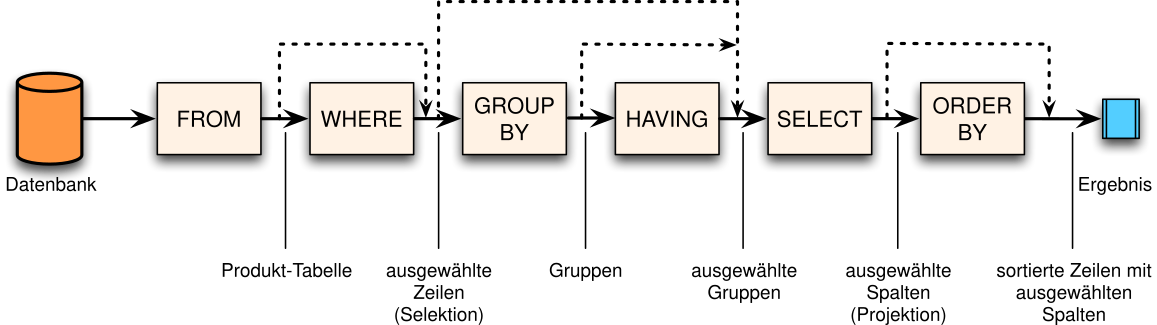
\includegraphics{images/sql-steps.png}
  \caption{Komponenten und sich ergebende Zwischenschritte bei der Verarbeitung einer \texttt{SQL}-Abfrage von Prof. Dr. Ulrich Hoffmann.}
  \label{fig:sql-steps}
\end{figure}

Einige der im folgenden beschriebenen Optionen sind redundant. Das liegt zum einen an \texttt{SQL} selbst, die Sprache sieht schlichtweg mehrere syntaktische Varianten für semantisch äquivalente Sachverhalte vor. Zum anderen könnte es aber auch aus didaktischen Gründen sinnvoll sein, die Wissensvermittlung mit einer Reihe von Spezialfällen zu beginnen.

\begin{enumerate}
\item \textbf{Projektionen mit \texttt{SELECT}} \\
  Diese Komponente als solche kann für Suchabfragen nicht ausgeschlossen werden. Außerdem muss mindestens \ref{feat:select-all} $\lor$ \ref{feat:select-column} erlaubt sein, sonst können keine gültigen \texttt{SQL}-Abfragen erstellt werden.
  \begin{enumerate}[noitemsep]
  \item \label{feat:select-all} Auswahl aller Spalten (``Sternchen-Operator'' \texttt{SELECT *})
  \item \label{feat:select-column} Auswahl von Spalten
  \item \label{feat:select-single-function} Ausdrücke aus einfachen Funktionsaufrufen zulassen
  \item \label{feat:select-simple-expression} Einfache Ausdrücke zulassen.
  \item \label{feat:select-expression} Beliebige Ausdrücke zulassen.
  \item \label{feat:select-distinct} Filterung des Ergebnisses auf unterscheidbare Daten (\texttt{DISTINCT}).
  \item \label{feat:select-limit} Beschränkung der Datenmenge mit \texttt{LIMIT}
  \end{enumerate}
\item \textbf{Angabe von Datenquellen mit \texttt{FROM}} \\
  Auch die Auslassung dieser Komponente ist nicht zulässig, obwohl einige \texttt{SQL} Dialekte dies durchaus erlauben. Im Rahmen von \idename{} wird dies aber nicht unterstützt: Die Schüler sollen \texttt{SQL} Abfragen grundsätzlich auf Tabellen beziehen und keine Daten ``aus der Luft greifen''\footnote{Für Oberflächen werden manchmal noch so etwas wie globale Konstanten benötigt, diese kommen dann aber nicht aus der \texttt{SQL}-Schicht.}.
  \begin{enumerate}[noitemsep]
  \item \label{feat:from-cross-join} Kreuzprodukt (\texttt{JOIN}) zulassen
  \item \label{feat:from-cross-comma} Kreuzprodukt (komma-separierte Schreibweise) zulassen
  \item \label{feat:from-natural-join} Automatische innere Verknüpfung zulassen (\texttt{NATURAL JOIN})
  \item \label{feat:from-inner-join} Innere Verknüpfung zulassen (\texttt{INNER JOIN}), erfordert \ref{feat:from-using} $\lor$ \ref{feat:from-on-simple}
  \item \label{feat:from-left-join} Linke äußere Verknüpfung zulassen (\texttt{LEFT OUTER JOIN}), erfordert \ref{feat:from-using} $\lor$ \ref{feat:from-on-simple}
  \item \label{feat:from-right-join} Rechte äußere Verknüpfung zulassen (\texttt{RIGHT OUTER JOIN}), erfordert \ref{feat:from-using} $\lor$ \ref{feat:from-on-simple}
  \item \label{feat:from-full-join} Volle äußere Verknüpfung zulassen (\texttt{FULL OUTER JOIN}), erfordert \ref{feat:from-using} $\lor$ \ref{feat:from-on-simple}
  \item \label{feat:from-using} \texttt{USING}-Bedingung zulassen
  \item \label{feat:from-on-simple} \texttt{ON}-Bedingung mit einfachen Ausdrücken zulassen
  \item \label{feat:from-on-expression} \texttt{ON}-Bedingung mit beliebigen Ausdrücken zulassen
  \item \label{feat:from-sub} Unterabfragen zulassen
  \end{enumerate}
\item \textbf{Filterung mit \texttt{WHERE} und \texttt{HAVING}} \\
  Da an dieser Stelle Ausdrücke zum Einsatz kommen, sind prinzipiell zwei unterschiedliche Ansätze denkbar. Zum einen die Verwendung einer vordefinierten Menge an Vergleichen mit einer einfachen Struktur, diese werden in \ref{sec:sql-subset-expression} beschrieben. Dem gegenüber steht der Ansatz fast beliebige Ausdrücke zu erlauben, was auf der einen Seite einen Ausbruch aus einem zu simplen Schema gleichkommen kann, auf der anderen Seite möglicher aber auch den Lernenden mit einem zu großen Freiheitsgrad überfordert.
  \begin{enumerate}[noitemsep]
  \item \label{feat:where-allow} \texttt{WHERE} zulassen
  \item \label{feat:having-allow} \texttt{HAVING} zulassen
  \item \label{feat:where-and} Verknüpfungen mit \texttt{AND}
  \item \label{feat:where-or} Verknüpfungen mit \texttt{OR}
  \item \label{feat:where-simple-expression} Einfachen Ausdrücke zulassen
  \item \label{feat:where-expression} Beliebige Ausdrücke zulassen
  \end{enumerate}
\item \textbf{Bildung von Gruppen mit \texttt{GROUP BY}}
  \begin{enumerate}[noitemsep]
  \item \label{feat:group-allow} \texttt{GROUP BY} zulassen
  \item \label{feat:group-multiple} Grupperierung mehrerer Spalten zulassen
  \end{enumerate}
\item \textbf{Sortierung mit \texttt{ORDER BY}} \\
  Bei dieser Komponente fehlt bewusst die Möglichkeit anhand eines Spaltenindexes aus dem \texttt{SELECT} zu sortieren. Da die gute Lesbarkeit der Abfragen ein erklärtes Ziel der Entwicklungsumgebung ist, wurde auf diese redundante Möglichkeit der Spaltenauswahl verzichtet.
  \begin{enumerate}[noitemsep]
  \item \label{feat:order-allow} \texttt{ORDER BY} zulassen, die Auswahl der Richtung (\texttt{ASC} und \text{DESC}) ist dann grundsätzlich möglich
  \item \label{feat:order-select} Sortierung nach im \texttt{SELECT} erwähnten Spalten oder Ausdrücken zulassen
  \item \label{feat:order-any-column} Sortierung nach beliebigen Spalten zulassen
  \item \label{feat:order-expression} Sortierung anhand eines beliebigen Ausdrucks zulassen
  \end{enumerate}
\end{enumerate}

\subsubsection{Mögliche Einschränkungen der Ausdrücke}
\label{sec:sql-subset-expression}

Nach dieser Betrachtung der mit der unmittelbaren \texttt{SQL}-Struktur zusammenhängenden Funktionalität ist es nun an der Zeit, sich den Ausdrücken ausführlicher zu widmen. Um eine graduelle Lernkurve sowie eine sinnvolle Unterstützung durch den Editor zu gewährleisten, werden diese in drei Klassen eingeteilt:

\begin{description}
\item[Einfache Ausdrücke] \hfill\\
  Einfache Ausdrücke unterliegen einer ganz festen Struktur, die nur sehr begrenzt die Schachtelung oder Verkettung von zusammengesetzten Ausdrücken zulässt. Ziel dieser Reduktion ist, dass die Auswertungsreihenfolge dieser Ausdrücke auch ohne die Verwendung von Klammern ``intuitiv'' eindeutig ist.

  Die Bearbeitung dieser Ausdrücke ist nicht notwendigerweise völlig frei, sondern könnte auch hinsichtlich der möglichen Operatoren oder der Struktur eingeschränkt werden.
\item[Komplexe Ausdrücke] \hfill\\
  Komplexe Ausdrücke lassen sich schachteln bzw. verketten und können mit einem Scratch-ähnlichen Editor für Ausdrücke frei bearbeitet werden. Die korrekte Beachtung von Auswertungsreihenfolgen ist Aufgabe der Lernenden, weswegen diese ggfs. die Ausdrücke auch selber Klammern müssen.

\item[Beliebige Ausdrücke] \hfill\\
  Beliebige Ausdrücke werden textuell notierte und vom \texttt{SQL}-Editor nicht weiter geprüft, sondern ungefiltert in die Abfrage eingesetzt werden. Sofern diese Art von Ausdrücken zugelassen wird erfolgt also auch keinerlei inhaltliche Einschränkung der zur Verfügung stehenden Möglichkeiten oder eine Syntaxüberprüfung.

  Diese Option soll es besonders fortgeschrittenen Lernenden erlauben, auch in nicht von \idename{} unterstützte Szenarien noch weiterarbeiten zu können. Damit wird verhindert, dass zu große Fortschritte der Lernenden \idename{} sofort obsolet machen.
\end{description}

Mit dieser Unterscheidung im Hinterkopf, können wir nun eine Menge an didaktisch sinvollen Einschränkungen definieren. Die Schüler sollen dabei durchaus auch Lernen, dass es sich bei Ausdrücken (nicht nur in \texttt{SQL}) um ein allgemeines Konzept handelt, welches Prinzipiell in der \texttt{SELECT}-Komponente genau so angewandt werden kann wie beim \texttt{ORDER BY}. Oder plastisch ausgedrückt: Wenn sich die Schüler aus didaktischen Gründen erstmal nur mit Ausdrücke im Rahmen der \texttt{SELECT}-Komponente beschäftigen sollen ist das eine sinnvolle, und daher mögliche Einschränkung. Nicht sinnvoll hingegen wäre es die Anwendung der \texttt{LENGTH(X)} Funktion nur in einer der beiden Komponenten zuzulassen. Letzteres wird daher auch nicht unterstützt.

\begin{enumerate}[resume]
\item \textbf{Allgemeine Optionen} \\
  Diese Optionen betreffen prinzipiell alle Stellen, an denen die entsprechenden Arten von Ausdrücken zugelassen werden.
  \begin{enumerate}[noitemsep]
  \item \label{feat:expr-allow-any-text} Ausdrücke als beliebigen Text zulassen, diese Option erlaubt die Umgehung aller Einschränkungen für einfache Ausdrücke!
  \item \label{feat:expr-allow-placeholder} An Stelle von Konstanten auch die Verwendung von Platzhaltern zur Bindung von Daten aus der Oberfläche zulassen.
  \end{enumerate}

\item \label{feat:expr-compute}  \textbf{Einfache Berechnende Ausdrücke} \\
  Diese Ausdrücke tauchen normalerweise in \texttt{SELECT}- oder \texttt{ORDER BY}-Komponenten auf, möglicherweise aber auch als Bestandteil eines einfachen Vergleichs.
  \begin{enumerate}[noitemsep]
      \item \label{feat:expr-compute-simple-func} Einfacher Funktionsaufruf mit Spalten oder Konstanten als Argument
      \item \label{feat:expr-compute-simple-arithmetic} Einfache Rechenausdrücke mit einer mathematischen Operation ($alter + 1$, $anzahl * preis$)
      \item \label{feat:expr-compute-simple-concat} Konkatenation von Strings\footnote{Sofern auch eine Oberfläche entwickelt werden soll, ist eine Konkatenation im Regelfall lieber dort vorzunehmen.}
  \end{enumerate}

\item \textbf{Einfache Vergleichende Ausdrücke} \\
  Diese ``typischen'' Vergleichsausdrücke sollten ausreichen um einen Großteil der nötigen Vergleiche in \texttt{WHERE}, \texttt{HAVING} und \texttt{ON} Komponenten abzudecken. Die linke Seite dieser Ausdrücke ist stets eine zur Verfügung stehende Spalte, der Vergleichsoperator und die rechte Seite eine der hier aufgezählten Möglichkeiten.

  Mit Vergleich ist dabei nicht nur der $=$-Operator gemeint, sondern auch die relationen Operatoren $\ne, <,\ge,\le$ und $>$. Die komplexeren Operatoren \texttt{LIKE} und \texttt{IN} sowie der ternäre Operator \texttt{BETWEEN} werden aber gesondert aufgeführt.

  \begin{enumerate}[noitemsep]
  \item \label{feat:expr-compare-const} Vergleich einer Spalte mit einem konstanten Wert
  \item \label{feat:expr-compare-null} Vergleich einer Spalte gegen \texttt{NULL}
  \item \label{feat:expr-compare-other-col} Vergleich einer Spalte mit einer anderen Spalte
  \item \label{feat:expr-compare-simple-func} Vergleich einer Spalte mit einem einfachem berechnenden Ausdruck (siehe \ref{feat:expr-compute})
  \item \label{feat:expr-compare-between} Test einer Spalte mit dem \texttt{BETWEEN}-Operator und zwei Konstanten
  \item \label{feat:expr-compare-like} Nutzung des \texttt{LIKE}-Operators mit einer Konstanten
  \item \label{feat:expr-compare-in} Nutzung des \texttt{IN}-Operators mit einer Liste von Konstanten
  \item \label{feat:expr-compare-negate} Negation aller einfachen Ausdrücke
  \end{enumerate}

\item \textbf{Allgemeine Funktionen (in alphabetischer Reihenfolge)} \\
  In einem Umfeld für Anfänger ist zu erwarten, dass fast jede Funktion (bzw. jede logische Gruppe an Funktionen) einer eigenen Einführung bedarf. Die Lehrkräfte sollen diese daher isoliert zur Verfügung stellen können, ohne Ablenkung durch nicht benötigte Funktionen.

  Bei unterschiedlich überladene Varianten der gleichen Funktion wird in \idename{} immer nur die vollständigste Variante implementiert. Die Schüler müssen daher nicht die implizit bekannten Werte der jeweiligen Funktion auswendig kennen.
  \begin{enumerate}[noitemsep]
  \item \label{feat:fun-abs} \texttt{ABS(X)} um den Betrag eines Wertes zu erhalten.
  \item \label{feat:fun-coalesce} \texttt{COALESCE(X,Y,...)} um den ersten gültigen Wert der Parameterliste zu erhalten.
  \item \label{feat:fun-length} \texttt{LENGTH(X)} um die Länge einer Zeichenkette zu bestimmen.
  \item \label{feat:fun-casing} \texttt{LOWER(X)} und \texttt{UPPER(X)} um die klein bzw. groß geschriebene Variante einer Zeichenkette zu erhalten.
  \item \label{feat:fun-random} \texttt{RANDOM()} um einen zufälligen Wert zu erhalten.
  \item \label{feat:fun-round} \texttt{ROUND(X,Y)} um kaufmännisch zu runden.
  \item \label{feat:fun-trim} \texttt{TRIM(X)} sowie \texttt{LTRIM(X)} und \texttt{RTRIM(X)} um Leerzeichen am Anfang oder Ende eines Strings zu entfernen.
  \item \label{feat:fun-substr} \texttt{SUBSTR(X,Y,Z)} um einen Ausschnitt der Zeichenketten zu extrahieren.
  \item \label{feat:fun-replace} \texttt{REPLACE(X,Y,Z)} um Teilbereiche der Zeichenkette zu ersetzen.
  \item \label{feat:fun-instr} \texttt{INSTR(X,Y,Z)} um das Vorkommen eines Suchwortes in einer Zeichenkette zu erhalten.
  \end{enumerate}

\item \textbf{Aggregierende Funktionen (in alphabetischer Reihenfolge)} \\
  Die Verfügbarkeit dieser Funktionen hängt von der Verfügbarkeit der \texttt{GROUP BY}-Komponente ab (\ref{feat:group-allow}).
  \begin{enumerate}[noitemsep]
  \item \label{feat:fun-avg} \texttt{AVG(X)} bildet das arithmetische Mittel.
  \item \label{feat:fun-count} \texttt{COUNT(X)} zählt alle Werte die nicht \lstinline{NULL} sind.
  \item \label{feat:fun-group-concat} \texttt{GROUP\_CONCAT(X,Y)} konkateniert einzelne Zellen einer Gruppe.
  \item \label{feat:fun-max-min} \texttt{MAX(X)} und \texttt{MIN(X)} selektieren minimalen oder maximalen Wert.
  \item \label{feat:fun-sum} \texttt{SUM(X)} summiert und gibt im Falle von komplett fehlenden Werten \texttt{NULL} zurück
  \item \label{feat:fun-total} \texttt{TOTAL(X)} summiert und gibt im Falle von komplett fehlenden Werten \texttt{0.0} zurück
  \end{enumerate}
\end{enumerate}

\subsubsection{Sprachstufen}
\label{sec:sql-subset-ranks}

Angelehnt an die bei Dr. Schemee bzw. Racket umgesetzte Idee der Feature-Levels \cite{macht-der-abstraktion} beschreibt dieses Kapitel konzeptionell, wie Lehrkräfte, aufbauend auf den im vorigen Kapitel beschriebenen Features, sinnvolle Untermengen von \texttt{SQL} definieren könnten, auf denen die mitgelieferten Beispielprojekte aufbauen. Bei den hier aufgeführten Beispielen handelt es sich keineswegs um die "`einzig korrekten"' Varianten. Vielmehr soll es für Lehrkräfte möglich sein, fast beliebige Teilmengen von \texttt{SQL} für ihre Schüler vorzugeben, nicht nur die im Rahmen dieser Arbeit als sinnvoll erachteten Kombinationen.

Das grundsätzliche Vorgehen um den Sprachumfang einzuschränken, ist dabei mehrstufig. Initial wird auf Projektebene mit einer Whitelist gearbeitet: Jede explizit erlaubte Funktionalität steht im \texttt{SQL}-Editor (siehe Kapitel \ref{sec:design-sql-editor} \nameref{sec:design-sql-editor}) zur Verfügung. Und sofern eine Funktionalität nicht erlaubt sein sollte, ist sie auch nicht verfügbar. Der Begriff ``Einschränkung'' ist aus der Sicht einer Whitelist also zwar nicht ganz optimal gewählt, beschreibt die stattfindende Reduktion des Umfangs von \texttt{SQL} aber akkurat.

Alternativ sollen sich auch wortwörtliche Einschränkungen im Sinne einer Blacklist angeben lassen. Für die in der Regel sehr übersichtlichen Teilsprachen die in dieser Arbeit konzipiert werden, ist diese Variante häufig schlechter lesbar: Man muss den größtmöglichen Umfang des hier beschriebenen Dialekts immer im Hinterkopf haben. Außerdem kommen im Falle einer Erweiterung des Sprachumfangs, z.B. durch ein späteres Update der Entwicklungsumgebung, möglicherweise unerwünschte Möglichkeiten hinzu.

Danach können die Einschränkungen noch für einzelne Abfragen verfeinert werden. Im allgemeinen Fall wird diese Funktionalität wenig nachgefragt sein: Insbesondere bei der Entwicklung von Webanwendungen ist es nicht hilfreich sich für jede Abfrage in einen anderen Sprachumfang einarbeiten zu müssen. Sofern die Schüler aber bestimmte Aufgaben mit einem didaktisch motiviertem reduzierten (oder erweiterten) Sprachumfang lösen sollen, kommt diese Möglichkeit zum Einsatz. Die hier exemplarisch aufgeführten Feature-Levels orientieren sich an den im Rahmen der Master-Arbeit exemplarisch erstellten Datenbeständen und an den Aufgaben aus Informatik-Lehrbüchern \cite{hubwieser_inf_2, grimm_informatik_2015}.

\begin{description}
\item[Arbeiten mit einfachen Einschränkungen] \hfill \\
  Die Selektion steht in allen betrachteten Schulbüchern am Beginn des Lernprozesses. Verwendet werden dabei durchgängig alle relationalen Operatoren ($<, \leq, =, \neq, \geq, >$) sowie das logische \lstinline{NICHT}, \lstinline{UND} sowie \lstinline{ODER}. Teilweise werden auch schon einfache unscharfe Textsuchen mit dem \lstinline{LIKE}-Operator behandelt. Syntaxzucker wie \lstinline{BETWEEN} kommt jedoch nicht vor.

\item[Arbeiten mit Projektionen] \hfill \\
  Der Funktionsumfang von diesem Feature-Level orientiert sich an gängigen Tabellenkalkulationsprogrammen wie Microsoft Excel oder Libre Office Calc. Im Vordergrund steht die Verwendung oder Schachtelung von Text-Funktionen wie \lstinline{substring} oder \lstinline{find}. Bei den Datensätzen handelt es sich häufig um stark denormalisierte Daten, welche nicht einmal in erster Normalform vorliegen. So werden zum Beispiel Vor- und Zuname in eine einzige Zelle geschrieben und müssen dann in der Projektion wieder voneinander getrennt werden.

\item[Arbeiten mit aggregierten Daten] \hfill \\
  Dieser Schritt ist gewissermaßen die logische Fortführung der Projektion. Die Lernenden müssen verstehen nach welchen Kriterien die Gruppierung erfolgen sollte und welche Spalten danach noch ohne Aggregation zur Verfügung stehen.

\item[Arbeiten mit JOINs] \hfill \\
  Dieses Feature-Level stellt die Verknüpfung vorhandener Datenbestände in den Vordergrund und blendet jegliche Projektion oder Gruppierung vollständig aus. Schüler sollen auf dieser Stufe lernen, sich in einem Datenmodell anhand der vorhanden Fremdschlüssel-Beziehungen zu orientieren.
\end{description}

\subsection{Drag \& Drop Editor für SQL}
\label{sec:design-sql-editor}

Der grafische Editor soll grundsätzlich ähnlich zu den aus Scratch bekannten Bedienkonzepten funktionieren können. Es kommen also distinkte Bedienelemente für die verschiedenen Komponenten einer \texttt{SQL} Abfrage zum Einsatz, kein reiner Texteditor. Der komponentenorientierte Editor soll dabei nicht die Konzeption von beliebigen Abfragen ermöglichen, wohl aber zumindest den Anforderungen aus Schulbüchern wie \cite{grimm_informatik_2015, hubwieser_inf_2} gerecht werden.

Grundsätzlich bedürfen einige Komponenten der Abfrage besonderer Aufmerksamkeit, weil sie große Auswirkungen auf das Verhalten der anderer Komponenten haben. Vorrangig ist hier die \texttt{GROUP-BY} Komponente zu nennen. Sobald die Query mit einer \texttt{GROUP BY} Komponente ausgestattet wird ist der Zugriff auf die konkreten Spalten einzelner Zeilen z.B. im allgemeinen Fall nicht mehr möglich. Das hinzufügen (oder entfernen) dieser Komponente hat also große Auswirkungen auf die Korrektheit der gesamten Abfrage. Ähnliches gilt für den Umgang mit \texttt{JOIN}s: Aus diesen leitet sich ab welche Daten von der Entwicklungsumgebung überhaupt angeboten werden sollten.

\subsubsection{Visuelle Gestaltung}

Für technische Details irrelevant, aber unbedingt ebenfalls im Voraus zu klären ist die Frage inwiefern es sinnvoll wäre, das sehr bunte, blockige Design von Scratch zu imitieren. Abbildung \ref{fig:compare-colourful} zeigt einen Vergleich zweier Prototypen aus der Konzeptionsphase von \idename{}: Einmal sehr bunt und ``blockig'' und einmal angelehnt an konventionelles Syntax-Highlighting.

\todo[inline]{\textbf{Todo}: Quelle mit Beleg für ``Kinderfreundliches'' buntes Design suchen. Das wird man bei Scratch schon aus gutem Grund gemacht haben. Relevante Frage: Zielgruppe (in Jahren) von Scratch vs. Zielgruppe dieses Projektes?}

\begin{wrapfigure}{r}{0.46\textwidth}
  \includegraphics[width=0.45\textwidth]{images/scratch-control-flow}
  \caption{Kontrollfluss in Scratch}
  \label{fig:screen-scratch-control-flow}
\end{wrapfigure}

Das blockige Design orientiert sich an Scratch und macht visuell sehr deutlich, welche Komponenten logisch zusammenhängen. Im Laufe der Entwicklung des Prototypen wurde aber immer deutlicher, dass die Zusammenhänge der Komponenten hier eher überbetont werden. In Scratch ist dieser deutliche visuelle Zusammenhang notwendig. So zeigen z.B. die Konnektoren der Blöcke für Ereignisse oder Endlosschleifen sehr deutlich, wie sich der Kontrollfluss durch diese Elemente verändern wird: Der Kontrollfluss beginnt mit dem Ereignis, ein Anhängen von Blöcken nach der Schleife ist weder möglich noch sinnvoll (Abbildung \ref{fig:screen-scratch-control-flow}).  Für eine vollständige Programmiersprache ist das mit Sicherheit eine gute Wahl, aber für den sehr linearen Ablauf einer \texttt{SQL}-Abfrage ist diese so ausgeprägte visuelle Hierarchie im Regelfall nicht nötig.

Die in den Prototypen noch zu sehende Nutzung von ``normalen'' Bedienelementen wie Text- oder Listboxen (Abbildung \ref{fig:compare-colourful} \& \ref{fig:screen-sql-editor-all-editing}) wurde schon früh in der Entwicklung zugunsten eines auf Drag \& Drop aufbauenden Konzeptes aufgegeben. Die Bedienelemente haben sich zum einen schon rein visuell die Lesbarkeit merklich gestört und hätten häufig ausgeblendet werden müssen. Zudem ist bei der Bearbeitung von Ausdrücken eine distinkte visuelle Hierarchie sehr von Vorteil. Diese Hierarchie lässt sich am einfachsten durch die konsequente Verwendung von klar kodierten Formen und Farben erreichen, was sich für vom Browser bereitgestellte Bedienelemente aber nur in engen Grenzen umsetzen lässt.

Darüber hinaus existiert noch ein weiterer Faktor, der zwar keinen Einfluss auf die technischen Details von \idename{} hat, aber trotzdem eine etwas ausführlichere Betrachung rechtfertigt: Die größere Nähe des etwas nüchterneren, IDE-ähnlichen Designs zu ``normalen'' Entwicklerprogrammen. Diese wirken möglicherweise weniger einschüchternd, wenn man sich schon an den Anblick von recht viel Text mit Syntax-Highlighting gewöhnt hat. Es ändert sich dann bei der Verwendung von ``echten'' Entwicklerprogrammen dann ``nur noch'' das Bedienparadigma sehr stark (Text schreiben statt Drag \& Drop), aber nicht mehr der visuelle Ersteindruck.

Letztendlich existiert aber auch noch ein sehr viel profanerer Faktor: Der Autor dieser Arbeit ist kein Grafikdesigner und würde ohne Hilfe vermutlich kein ansprechendes, durchgehend ``blockiges'' Gesamtkonzept auf die Beine stellen können. Das endgültige Design lehnt sich bei dem Editor für Ausdrücke durch die Verwendung von Blöcken also visuell an Scratch an, nutzt zur Visualisierung der Komponenten jedoch eine an Syntax-Highlighting orienierte Darstellung.

\begin{figure}[h]
  \begin{subfigure}[b]{0.45\textwidth}
    \includegraphics[width=\textwidth]{images/sql-sketch-early-colourful}
    \caption{Starke Betonung der Blöcke}
    \label{fig:screen-sql-editor-early-colourful}
  \end{subfigure}\hfill
  \begin{subfigure}[b]{0.45\textwidth}
    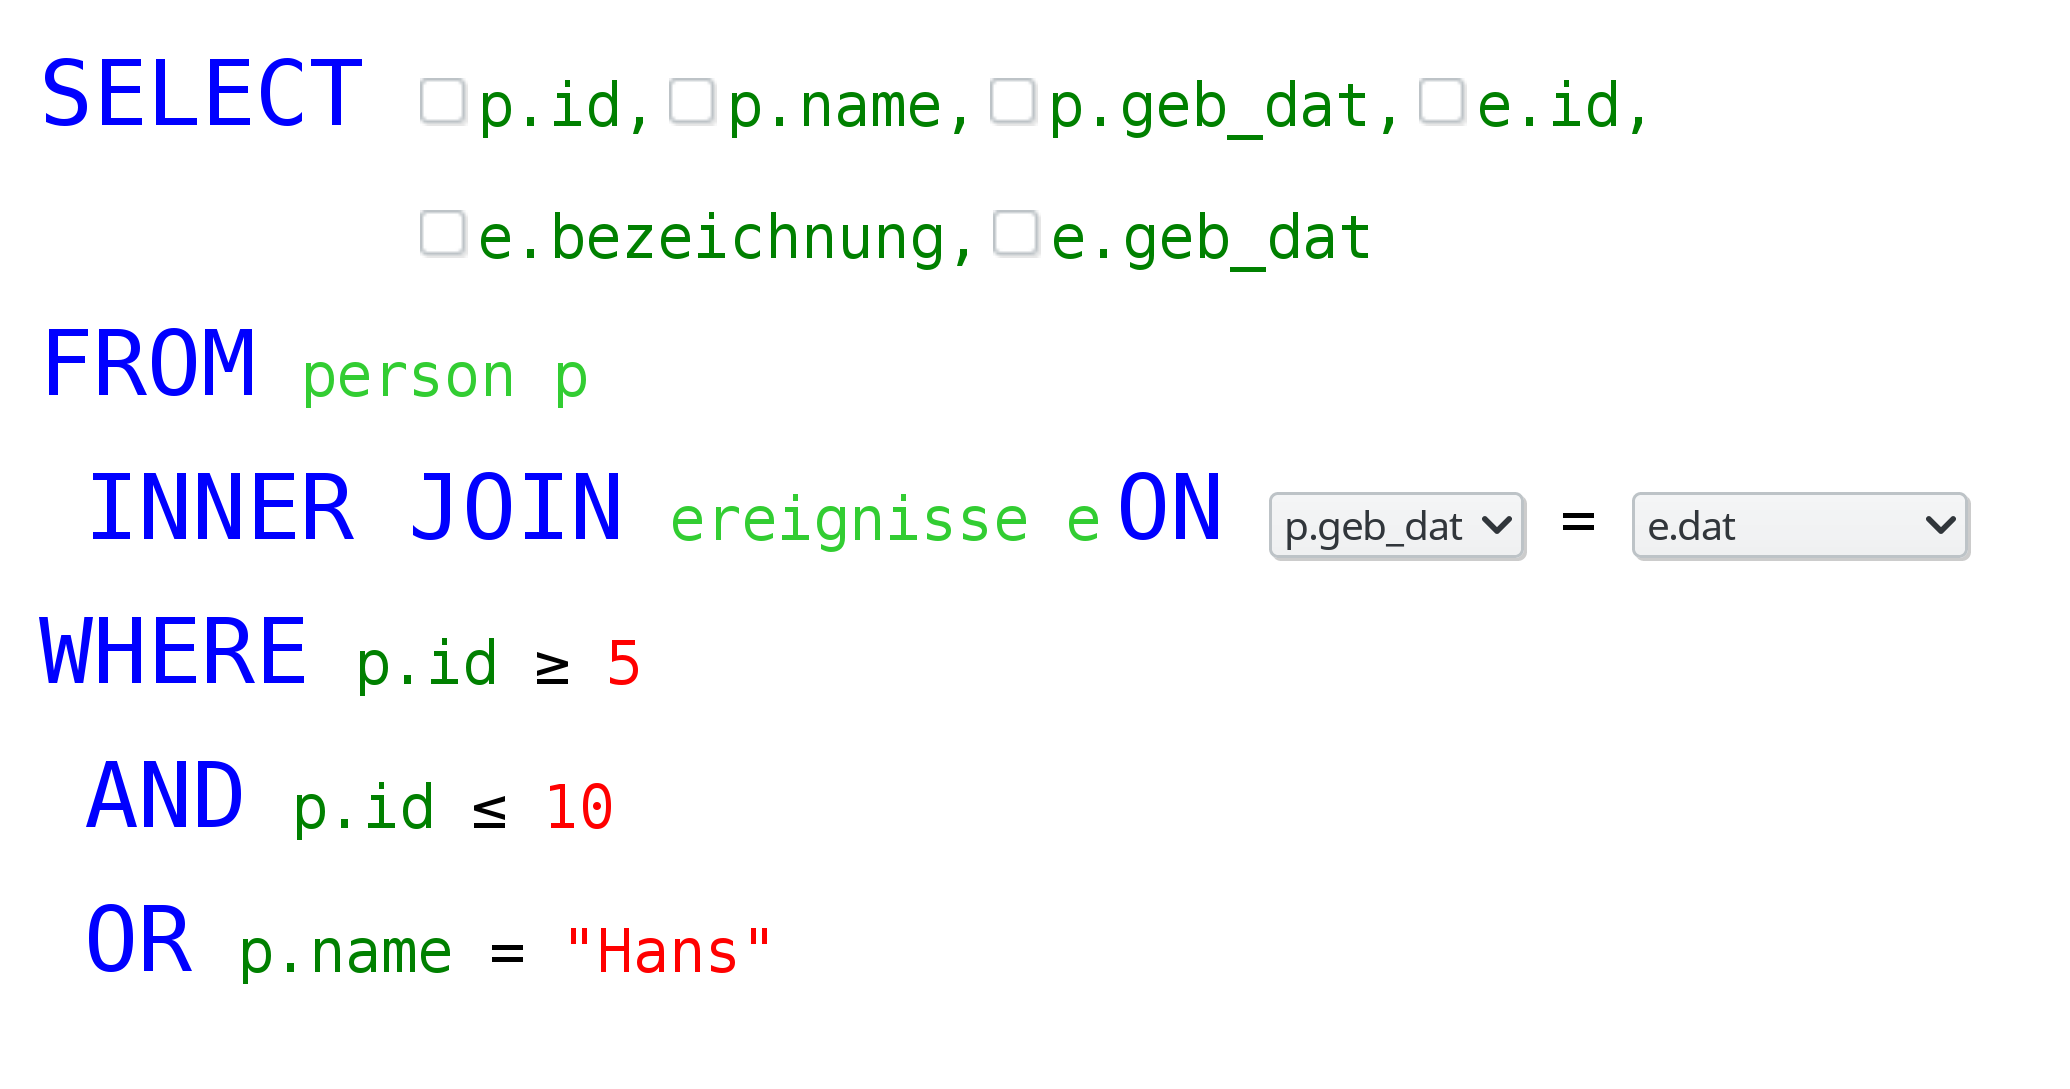
\includegraphics[width=\textwidth]{images/sql-sketch-early-syntax-highlight}
    \caption{Syntax-Highlighting}
    \label{fig:screen-sql-editor-early-syntax-highlighting}
  \end{subfigure}
  \caption{Vergleich unterschiedlicher Gestaltungsansätze}
  \label{fig:compare-colourful}
\end{figure}

\subsubsection{Grundsätzlicher Aufbau}

Es stellt sich zunächst die Frage, ob der Editor, wie Scratch, mit einer Drag \& Drop Seitenleiste ausgestattet werden sollte, oder ob auch ein anderes Bedienkonzept denkbar wäre. Ein grundsätzlicher Nachteil Drag \& Drop Bedienkonzeptes ist der nötige Platz für die Unterbringung aller verwendbaren Komponenten. Spätestens wenn für die Anzeige aller verfügbaren Optionen nicht ausreichend Platz auf dem Bildschirm vorhanden ist, muss sorgfältig geplant werden, wie die entsprechenden Bedienelemente anzuordnen sind.

Scratch nutzt eine Einordnung der Blöcke in zehn Kategorien. Es sind daher nie alle existierenden Blöcke auf einmal sichtbar, sondern immer die thematisch verwandten Blöcke der aktuell gewählten Kategorie. Eine solche Kategorisierung muss sehr sorgfältig entwickelt und vor allem erprobt werden: Sollten die Zuordnung eines Blocks mehrdeutig oder mißverständlich sein besteht die Gefahr, dass er nicht gefunden wird. Im Rahmen dieser Arbeit würde diese Problematik der Kategorisierung daher erst einmal verschoben: Es wird darauf verzichtet, solange die zur Verfügung stehenden Bedienelemente noch bequem Platz in einem Full-HD-Browserfenster haben.

Da der Benutzer immer nur eine Abfrage zur Zeit bearbeiten können soll, ergibt sich der einzig mögliche Platz für viele Blöcke automatisch. Darüber hinaus ist die Reihenfolge eines Großteils der Komponenten einer Abfrage sehr strikt festgelegt, so kann eine \texttt{GROUP BY} Komponente nicht an beliebigen Stellen verwendet werden, sondern nur nach der \texttt{FROM} oder der \texttt{WHERE} Anweisung. Andere Komponenten wie z.B. \texttt{HAVING} oder logische Verknüpfungen mit \texttt{AND} oder \texttt{OR} sind nicht nur von der Reihenfolge, sondern auch von der Existenz anderer Bestandteile abhängig. Ein möglicher Ansatz zur Reduktion der verfügbaren Komponenten wäre also, die möglichen Optionen visuell abgegrenzt Platzhalter innerhalb des Abfrageeditors anzubieten. Ein Klick auf den Platzhalter könnte diesen dann in einen konkreten Block umwandeln und gegebenenfalls zur Angabe der benötigten Parameter auffordern.

\begin{figure}[p]
  \includegraphics[width=\textwidth]{images/sql-sketch-all-editing}
  \caption{So nicht! Ohne Nutzung von Drag \& Drop und daher simultane Anzeige (fast) aller Möglichkeiten, zudem ausgiebige Nutzung von "`normalen"' Bedienelementen.}
  \label{fig:screen-sql-editor-all-editing}
\end{figure}

Im Rahmen der vorab entwickelten, rein visuellen Prototypen hat sich herausgestellt, dass eine permanente Anzeige aller Editierungsmöglichkeiten mit einem sehr überladen wirkenden Benutzerinterface einher geht, insbesondere was die Einblendung von Platzhaltern angeht. Abbildung \ref{fig:screen-sql-editor-all-editing} zeigt einen Screenshot eines Prototypen, bei dem nahezu alle denkbaren Editierungsoptionen gleichzeitig für den Lernenden verfügbar sind und daher angezeigt werden müssen. Trotz der klaren visuellen Unterscheidung fällt es schwer mit nur einem Blick zu erkennen, was die Abfrage jetzt tatsächlich beinhaltet.

Statt jederzeit alle Optionen anzuzeigen, könnte dann noch die Position des Mauszeigers herangezogen um zu entscheiden, welche Platzhalter angezeigt werden sollen. So wurden alle Editierfunktionen ausgeblendet, wenn sich die Maus außerhalb der Abfrage befand, die \texttt{JOIN}-Optionen nur gezeigt, wenn der Cursor sich gerade in der Nähe befand, ... Das Ergebnis war allerdings eine Benutzerschnittstelle, deren Bedienelemente häufig und für einen ungeübten Benutzer auch unerwartet ihre Position verändert haben. Dementsprechend wurde dieser Ansatz noch in der Konzeptionsphase verworfen. Darüber hinaus hätte man mit diesem Ansatz nur hierarchisch verwandte Bereiche ausblenden können: Für die \texttt{GROUP BY}-, \texttt{ORDER BY}- oder \texttt{UNION}-Platzhalter ergibt sich keine intuitive Position des Mauszeigers, bei der diese kontextsensitiv eingeblendet werden könnten.

Das endgültig implementierte Design (Abbildung \ref{fig:screen-sql-editor-drag-drop}) lehnt sich nun doch an Scratch an, versucht allerdings mit Platzhaltern den Benutzer kontextsensitiv zu unterstützen. Wenn dieser zum Beispiel einen Vergleichsoperator für Ausdrücke in der Seitenleiste anwählt, werden im Hauptfenster die validen Drop-Ziele hervorgehoben. Unter dem eigentlichen Editor befinden sich dann zwei weitere Bereiche (Abbildung \ref{fig:screen-sql-editor-parameters-preview}): Zum einen die Ergebnisanzeige, welche die zur aktuellen Gestalt der Abfrage passenden Zeilen zeigt. Und zum anderen eine Möglichkeit, bei Abfragen mit Parametern die nötigen Werte zu definieren. Und an dieser Abbildung wird ein weiteres Detail deutlich: Abfragen lassen sich nur als "`einzeilig"' deklarieren, wenn eine \texttt{WHERE}-Komponente vorhanden ist.

\begin{figure}[h]
  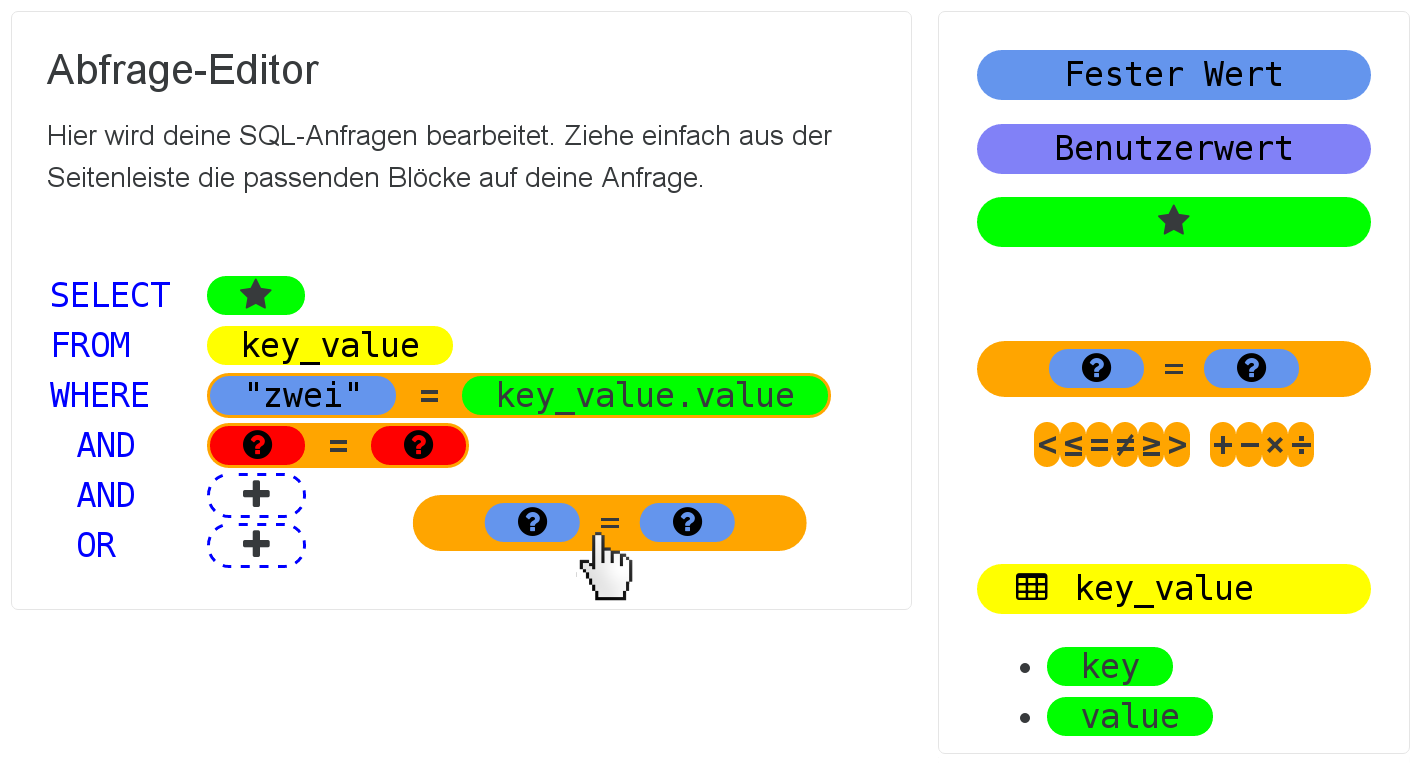
\includegraphics[width=\textwidth]{images/sql-drag-drop}
  \caption{Stattdessen: Drag \& Drop Interface mit Hervorhebung von möglichen Zielen beim Ziehen aus der Seitenleiste, keine Nutzung von "`normalen"' Bedienelementen.}
  \label{fig:screen-sql-editor-drag-drop}
\end{figure}

\begin{figure}[p]
  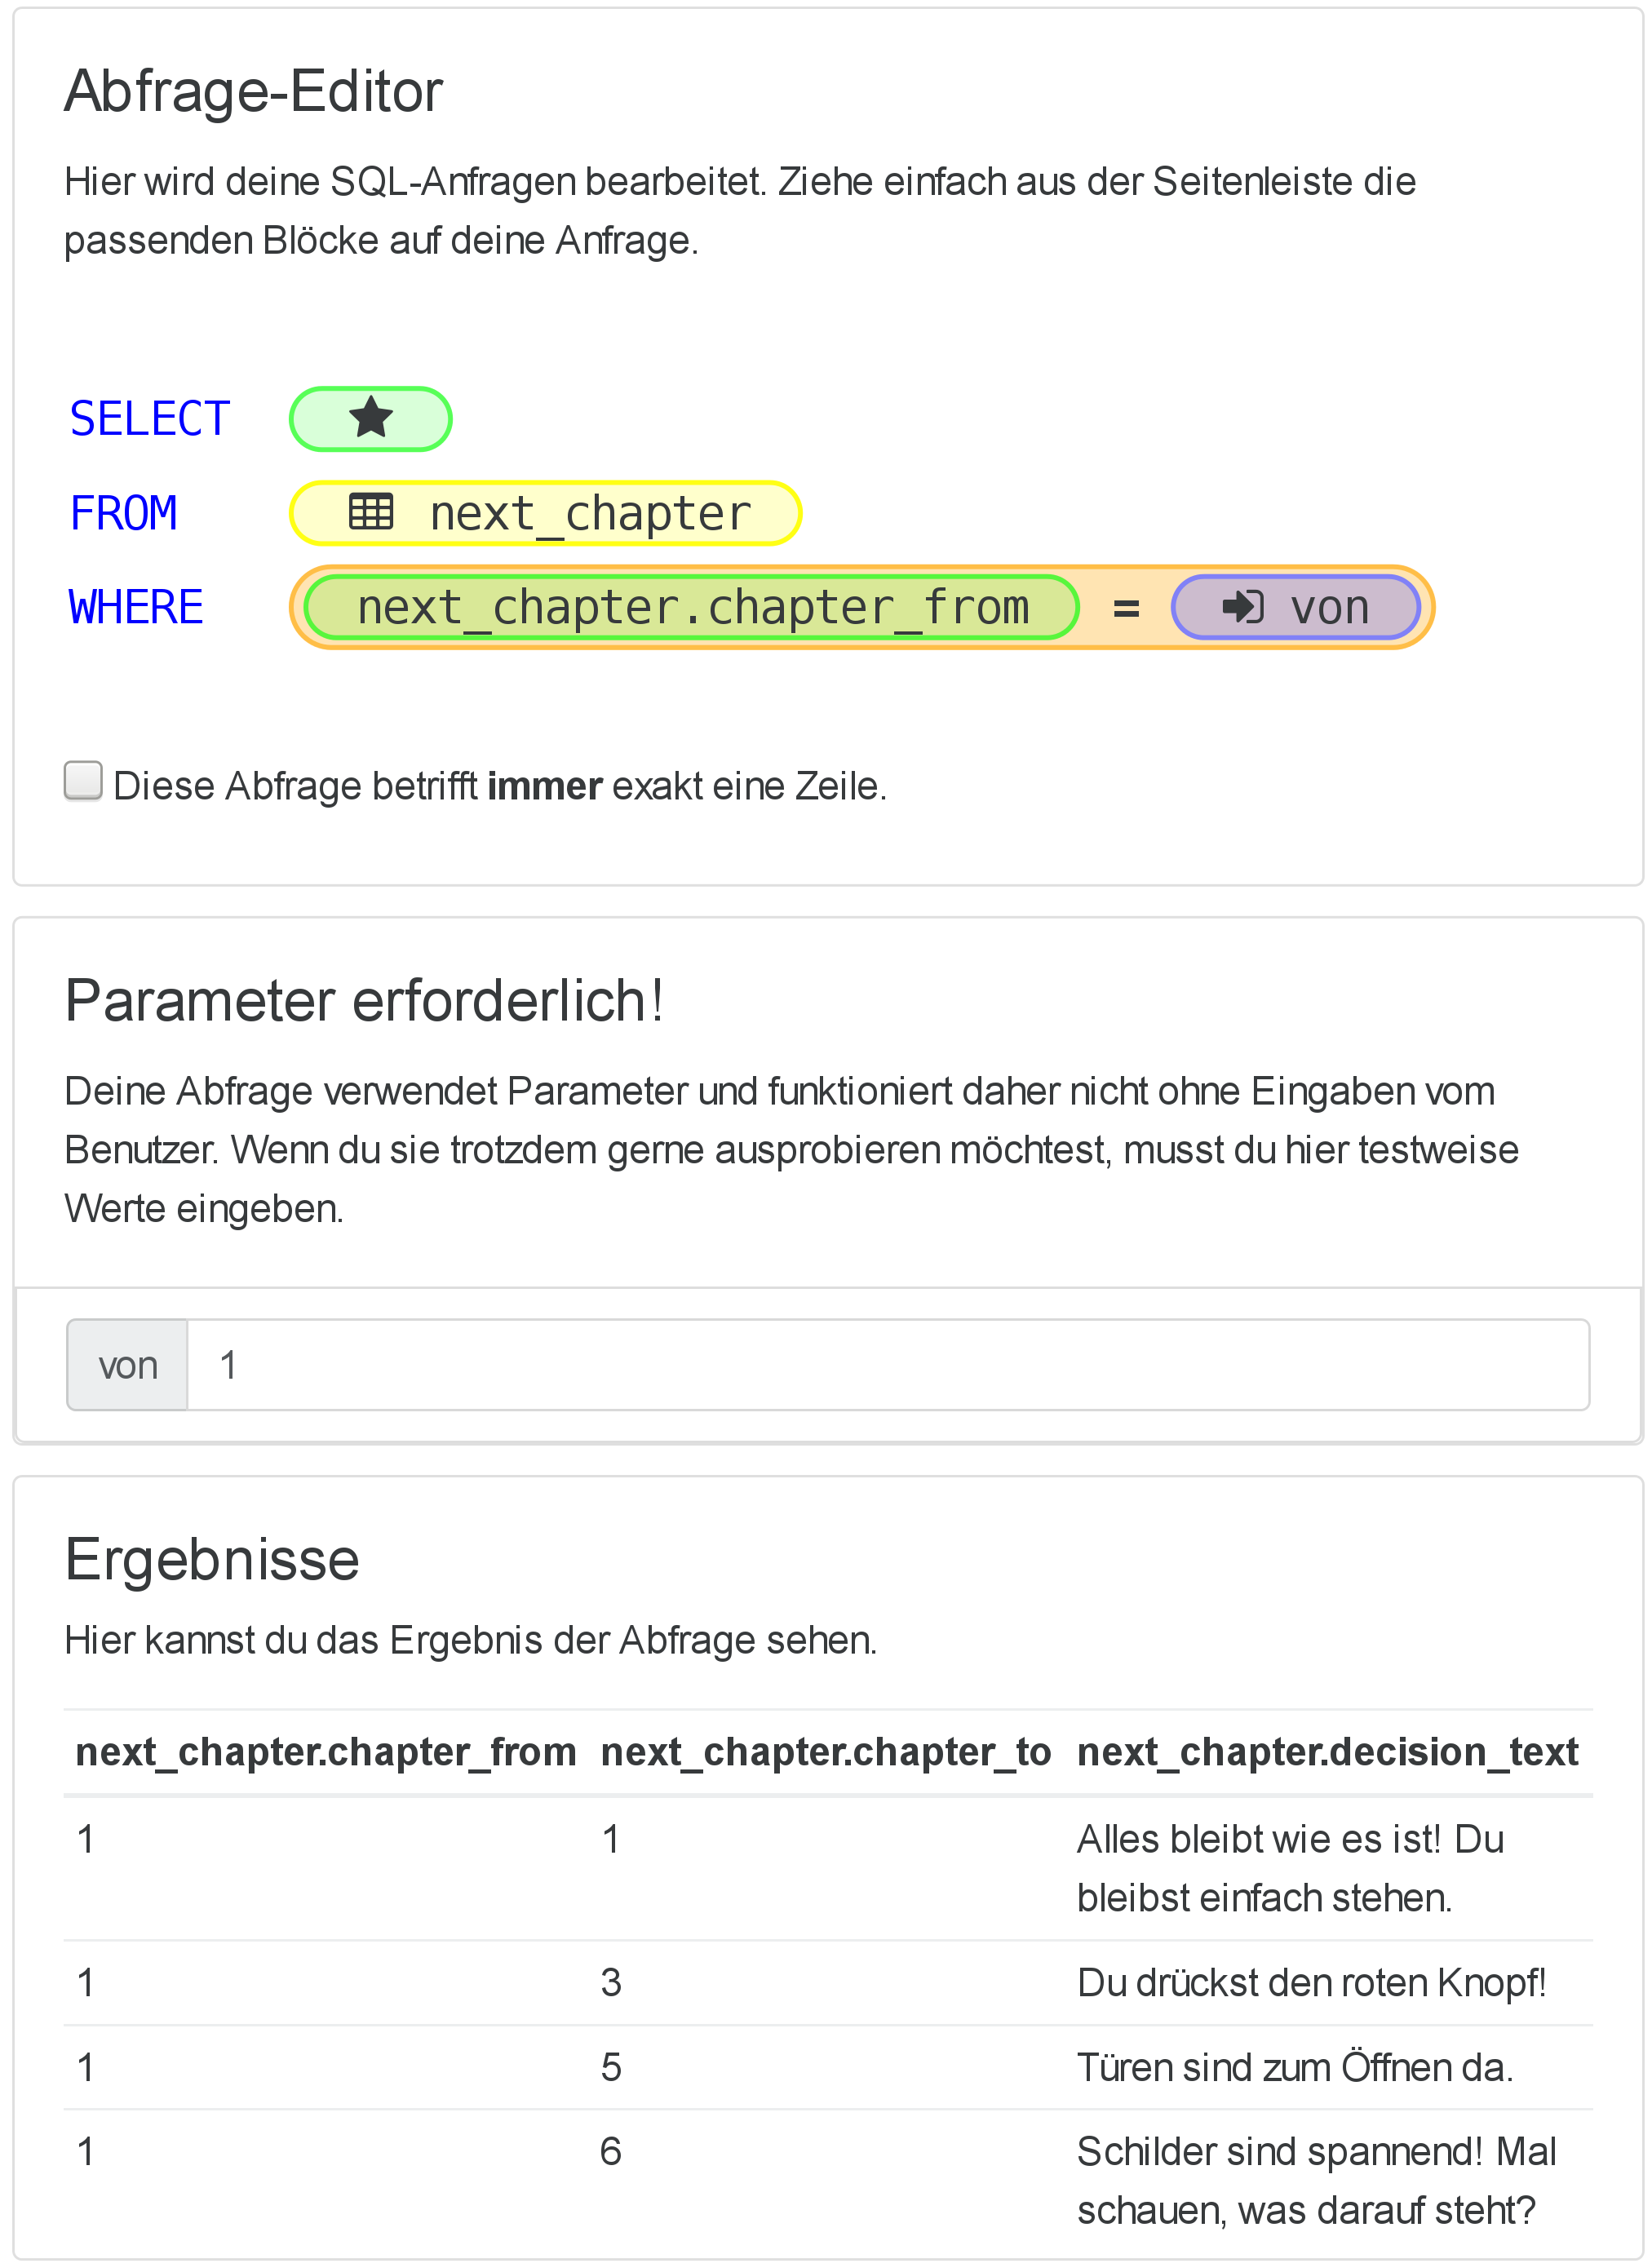
\includegraphics[width=\textwidth]{images/sql-parameters-preview}
  \caption{Abfrageeditor: Parameter für eine parametriesierte Abfrage und Ergebnisvorschau}
  \label{fig:screen-sql-editor-parameters-preview}
\end{figure}

\subsubsection{Umgang mit Ausdrücken}

Innerhalb der \texttt{SELECT}- und \texttt{WHERE}-Komponenten können theoretisch beliebige Ausdrücke auftreten. Diese unterscheiden sich ganz wesentlich anhand ihrer benötigten Parameter. Konstanten, Spalten und "`Benutzerwerte"' stehen für sich, können also unmittelbar verwendet werden. Sofern Ausdrücke andere Ausdrücke zur Auswertung benötigen, zum Beispiel das logische \texttt{UND}, werden diese zunächst durch einen speziellen "`hier fehlt etwas"'-Platzhalter gefüllt. Auf diesen Platzhalter, symbolisiert durch ein Fragezeichen, lassen sich dann wie gewohnt per Drag \& Drop andere Ausdrücke der Abfrage oder Elemente aus der Seitenleiste ziehen.

Aus Zeitgründen wurde die Unterstützung für einfache Ausdrücke zunächst einmal zurückgestellt. Schon die Fragestellung, ob diese Vereinfachung lieber die Inhalte in der Seitenleiste reduzieren oder in einem neuen Dialog stattfinden sollte wirft eine Vielzahl von grundsätzlichen Problemen auf: Sollen für komplexe Sachverhalte eigene "`Untereditoren"' entwickelt werden? Auch wenn diese aus didaktischer Sicht möglicherweise hilfreich wären, stellt sich die Frage ob das Drag \& Drop Paradigma dafür durchbrochen werden sollte. Und da sich mit dem Drag \& Drop Ansatz alle Ausdrücke entwerfen lassen, wurde die Diskussion über die geeignetste Implementierung dieser Funktion verschoben.

\subsubsection{Abfragen mit Parametern}
\label{sec:design-query-params}

Um eine Interaktion mit Endbenutzern zu ermöglichen können in Ausdrücken auch benannte Parameter ("`Benutzerwerte"') anstelle von konstanten Werten verwendet werden. Im Gegensatz zu Konstanten werden diese zur Laufzeit vom Benutzer angegeben. Aus Sicht der \texttt{SQL}-Abfrage ist diese Ergänzung relativ trivial, schließlich sind benannte Parameter Teil faktisch jeder \texttt{SQL}-Implementierung. Die eigentliche Problematik liegt im Binden dieser Parameter zur Laufzeit. Das Kapitel \ref{sec:design-ui-editor} beschreibt den Editor für Benutzeroberflächen, durch welchen die Verknüpfung mit den Bedienelementen der Oberfläche vorgenommen wird.

Innerhalb des Abfrageeditors können solche parametrisierten Abfragen dann natürlich nicht mehr direkt ausgeführt werden. Auf diesen Umstand wird der Entwickler, wie in Abbildung~\ref{fig:screen-sql-editor-parameters-preview} zu sehen ist, direkt innerhalb des Editors hingewiesen.

\subsubsection{\texttt{FROM}}

Wenn der Benutzer eine Drag-Operation mit einer Tabelle beginnt, kann er die Tabelle wahlweise auf einer bestehenden Tabelle "`fallen lassen"', einen $\bigoplus$-Indikator nach der letzten Tabelle oder den \texttt{FROM}-Text selbst fallen lassen. Eingefügt wird dabei im Falle von schon existierenden Elementen immer nach dem Ziel, die $\bigoplus$-Indikatoren werden hingegen einfach durch das neue Element ersetzt.

Diese Komponente beinflusst unmittelbar die in der Seitenleiste zur Verfügung stehenden Daten. Für Tabellen, die bisher nicht als Teil der \texttt{FROM}-Komponente sind, stehen die Spalten nämlich nicht zur Verfügung. Erst wenn man diese Tabelle mit einem \texttt{JOIN} in die Abfrage einbindet, erscheinen auch die dazugehörigen Spalten in der Seitenleiste.

\subsubsection{\texttt{WHERE}}

Sobald eine Drag-Operation mit einem Ausdruck beginnt, wird entweder die \texttt{WHERE}-Komponente mit einem $\bigoplus$-Indikator eingeblendet oder, im Falle von schon existierenden Einschränkungen, die \texttt{AND}- und \texttt{OR}-Operatoren, ebenfalls mit einem $\bigoplus$-Indikator. Der letztere Fall wird in Abbildung~\ref{fig:screen-sql-editor-drag-drop} illustriert.

Syntaktisch gesehen wären die logischen Verknüpfungen natürlich auch als Teil der "`normalen"' binären Ausdrücke möglich. In der Praxis wird der Quelltext von \texttt{SQL}-Abfragen allerdings häufig anhand dieser Verknüpfungen umgebrochen. An dieser Stelle folgt \idename{} also einer bewährten Konvention, auch wenn das syntaktisch nicht unbedingt notwendig wäre.

\subsubsection{\texttt{GROUP BY}}

Sobald in einer Abfrage eine \texttt{GROUP BY} Komponente auftaucht, hat dies Auswirkungen auf die Möglichkeiten innerhalb der \texttt{SELECT} Anweisung. Da keine Auswahl von ungruppierten und nicht-aggregierten Spalten möglich sein darf, müssen diese entfernt werden. Insbesondere wenn der Benutzer vorher schon mit komplizierten Ausdrücken im \texttt{SELECT} gearbeitet haben sollte, ist also zumindest eine Warnung nötig.

\subsubsection{Manipulation von Daten}

Neben den bisher ausführlich besprochenen \texttt{SELECT}-Anweisungen müssen sich natürlich \texttt{INSERT}-, \texttt{UPDATE}- und \texttt{DELETE}-Anweisungen umsetzen lassen. Da diese ihrer Natur nach nicht idempotent sind verbietet sich natürlich eine wiederholte, automatische Ausführung während der Entwicklungszeit. Es ist zu erwarten, dass die meisten von den Schülern verfassten Abfragen dieser Art ausführlichen Gebrauch von den in Kapitel \ref{sec:design-query-params} beschriebenen Parametern machen.

Die Ausführung dieser Operation sollte daher immer in zwei Schritten erfolgen, die von einer Vorschau auf das Ergebnis begleitet werden. Erst wenn diese Ergebnisvorschau vom Entwickler bestätigt wird, werden die Änderungen tatsächlich übernommen. Für \texttt{DELETE}- und \texttt{INSERT}-Operationen kann diese Vorschau einfach den kompletten neuen bzw. zu löschenden Datensatz anzeigen. Im Falle von \texttt{UPDATE}-Anweisungen sollten alle veränderten Datensätze einander gegenübergestellt werden.

\begin{figure}[h]
  \includegraphics[width=\textwidth]{images/sql-insert-key-value-pairs}
  \caption{Abfrageeditor: Anderes Erscheinungsbild für Spalte-Wert-Paare, wie sie bei \texttt{INSRT} oder \texttt{UPDATE} Operationen nötig sind}
  \label{fig:screen-sql-editor-insert-key-value-pairs}
\end{figure}

Für die Name-Wert-Paare in \texttt{INSERT}- oder \texttt{UDPATE}-Operationen löst sich das Erscheinungsbild des Editors von dem Vorbild der \texttt{SQL}-Syntax (Abbildung  \ref{fig:screen-sql-editor-insert-key-value-pairs}). Zur Erinnerung werden an dieser Stelle noch einmal die SQLite-Syntax für \texttt{UPDATE}- und \texttt{INSERT}-Anweisungen illustriert (Listing \ref{lst:sql-syntax-insert} \& \ref{lst:sql-syntax-update}). Leider haben diese beiden verwandten Anweisungen offensichtlich eine unterschiedliche Syntax für die Notation der Schlüssel-Wert-Paare.\footnote{Dieser Umstand wurde mit SQLite Version 3.15.0 für die \texttt{UPDATE}-Anweisung verbessert. Es ist nun auch möglich auf beiden Seiten der Zuweisung identisch lange Listen von Spalten und Werten anzugeben. Allerdings ist Version 3.15.0 am 14. Oktober 2016 erschienen, etwa eine Woche vor dem Druck dieser Thesis.}. Dieses syntaktische Detail der wird vor dem Entwickler durch die Oberfläche versteckt: Sichtbar ist dort nur die abstrakte Zuweisung von Werten an eine Auswahl von Spalten.

\begin{lstlisting}[language=SQL,float=h!,caption={Syntax einer \texttt{INSERT}-Anweisung}, label={lst:sql-syntax-insert}]
INSERT INTO gefangen (pokedex_nummer, spitzname, staerke)
VALUES (:nummer, :name, :staerke)
\end{lstlisting}

\begin{lstlisting}[language=SQL,float=h!,caption={Syntax einer \texttt{UPDATE}-Anweisung}, label={lst:sql-syntax-update}]
UPDATE gefangen
SET spitzname = :neuer_name, staerke = :neue_staerke
WHERE gefangen_id = :geaendertes_pkmn;
\end{lstlisting}

Um zwischen bewusst und versehentlich nicht vom Entwickler gesetzten Werten zu unterscheiden ist in der aktuellen Fassung leider noch die Nutzung einer Checkbox vorgesehen. Das ist ein Bruch mit dem üblicherweise verwendeten Drag \& Drop-Paradigma und sollte in einer künftigen Version durch aus der Seitenleiste ziehbare Spalten abgelöst werden.

\subsection{Konzept für Oberflächen}
\label{sec:design-ui-concept}

\warning{Diese Oberflächen werden nicht ausschließlich in normalem HTML verfasst, es kommen noch einige Erweiterungen in Form einer Templatingengine zum Einsatz. Ähnlich wie für die \texttt{SQL}-Abfragen wird also auch für die Oberflächen ein dezidierter Editor (Kapitel \ref{sec:design-ui-editor}) implementiert. Die Schüler sollten zu keinem Zeitpunkt selber Quelltexte tippen müssen, optional aber durchaus die Möglichkeit dazu haben.}

Damit sich mit der Schülerentwicklungsumgebung erstellte Projekte auch von normalen Endanwendern bedienen lassen, bedarf es natürlich noch der entsprechenden Benutzeroberfläche. Hier bietet sich, aus Gründen der einfachen Weitergabe, eine webbasierte Oberfläche an: Dadurch entfällt bei den Endanwendern jegliche Installation und gerade für datenzentrierte, verteilte Anwendungen ist eine einheitliche Sicht auf den Datenbestand von großer Bedeutung. Ein weiterer positiver Aspekt ist die einfache Weitergabe der eigenen Arbeitsergebnisse: Diese können über eine beliebige soziale Plattform durch Weitergabe einer \texttt{URL} mitgeteilt werden.

Abstrakt betrachtet besteht eine \idename{}-Seite aus zwei wesentlichen Informationen: Eine Auflistung aller zum Darstellen benötigten Datenquellen, im Rahmen dieser Thesis werden das ausschließlich \texttt{SQL}-Abfragen sein, und eine Vorschrift wie genau dieser Datenbestand darzustellen ist.

Um das folgende Kapitel anschaulicher zu gestalten, werden alle Beispiele anhand eines sehr reduzierten Datenbestandes (siehe Tabelle \ref{tab:ui-concept-data-article} \& \ref{tab:ui-concept-data-comment}) zu einem einfach Blog illustriert. Dieser besteht aus zwei Tabellen für Artikel und Kommentare, ein Artikel wurde dabei möglicherweise mehrfach kommentiert. Bei den Zeitangaben handelt es sich um \texttt{UNIX}-Zeitstempel.

\begin{table}[h]
  \centering
  \begin{tabularx}{\linewidth}{ l l X l }
    article\_id&caption&text&date\\
    \hline
    1&Erster Artikel&In dem noch nicht besonders viel Text steht.&1393423200\\
    2&Nächster Artikel&Hier steht schon ein bisschen mehr.&1456498800\\
    3&Dritter Artikel&<abbr title="'Hypertext Markup Language"'>HTML</abbr>&1477872000\\
  \end{tabularx}
  \caption{\texttt{article}-Daten des Blog-Beispiels}
  \label{tab:ui-concept-data-article}
\end{table}

\begin{table}[h]
  \centering
  \begin{tabularx}{\linewidth}{ l l l X l }
    comment\_id&article\_id&commenter\_name&text&date\\
    \hline
    1&1&Ash Ketchum&Hast du schon meine Pokemon-Seite gesehen?&1393423241\\
    2&1&Betreiber&Natürlich, gute Arbeit!&1393435123\\
    3&3&Kommentator&Auch <strong>dieser Kommentar</strong> enthält HTML.&0\\
  \end{tabularx}
  \caption{\texttt{comment}-Daten des Blog-Beispiels}
  \label{tab:ui-concept-data-comment}
\end{table}

Dieser Blog soll dem Endbenutzer über zwei Seiten näher gebracht werden: Eine \textit{Hauptseite} dient der Auflistung aller Blogbeiträge welche im Einzelnen auf einer \textit{Detailseite} in Gänze betrachtet und kommentiert werden können. Dabei können auf der Hauptseite natürlich nicht die gleichen Informationen angezeigt werden, diese werden daher teilweise aggregiert: Statt alle Kommentare zu einem Beitrag anzuzeigen, wird nur auf die Anzahl der getätigten Kommentare verwiesen.

Bei dieser Aufteilung handelt es sich um eine typische "`Master-Detail"'-Struktur: Ausgehend von einer sehr komprimierten Darstellung aller Werte können Details zu einem konkreten Datensatz nach einem Navigationsvorgang eingesehen werden. Dieses Navigationskonzept wird von fast allen geschäftlichen Applikationen genutzt und ist eine der Standardvorlagen des Visual Studio Lightswitch.

\subsubsection{Datenquellen für Webseiten}

Um die einer Webseite zur Verfügung stehenden Daten zu strukturieren, wird der verfügbare Datenbestand in unterschiedliche Namensräume eingeteilt. Dadurch werden Kollisionen von Bezeichnern vermieden und es ist schon anhand der Bezeichnung eindeutig, von welchem Kontext der Wert zur Verfügung gestellt wird.

\begin{description}
\item[\texttt{page} für Eigenschaften der Seite] \hfill \\
  Zumindest der Name der aktuellen Seite ist für die Darstellung möglicherweise relevant und sollte daher während des Rendervorgangs zur Verfügung stehen.
\item[\texttt{project} für Eigenschaften des Projektes] \hfill \\
  Wenn man als Entwickler globale Konstanten ablegen möchte, könnte man dies natürlich auch in der Datenbank tun. Bequemer ist aber ein separater Speicherort, der tatsächlich keine Modifikationen durch Endbenutzer vorsieht. Das typische Beispiel für einen solchen global verfügbaren Wert wäre der Name des Projekts an sich.
\item[\texttt{get} für \texttt{URL}-Parameter] \hfill \\
  Wenn aus einer Vielzahl von verfügbaren Daten zu einem bestimmten Datensatz navigiert werden soll, sieht der \texttt{HTML}-Standard die Verwendung von \texttt{URL}-Parametern vor. Mit diesen lassen sich applikationsspezifische Merkmale der anzuzeigenden Datensätze angeben. Im Falle des Blog-Beispiels wäre das zum Beispiel die \texttt{article\_id} zur Anzeige eines bestimmten Beitrages oder die Angabe eines Startzeitpunkts um die Hauptseite in mehrere Seiten zu unterteilen.
\item[\texttt{query} für \texttt{SELECT}-Abfragen] \hfill \\
  Nicht jede Webseite benötigt notwendigerweise die Ergebnisse aller verfügbaren Abfragen. Daher werden die tatsächlich benötigten referenzierten Abfragen in diesem Namensraum gesammelt. Kapitel \ref{sec:design-ui-bind-output}~\nameref{sec:design-ui-bind-output} beschreibt im Detail wie diese Anbindung funktioniert.
\item[\texttt{input} für Benutzereingaben] \hfill \\
  Dieser Namensraum hängt eng mit dem HTML-\texttt{form}-Element zusammen und stellt die Werte aller Benutzereingaben zur Verfügung.
\end{description}

Die Verwendung von Namensräume ist von Jekyll inspiriert, \texttt{page} und \texttt{project} findet man auch dort. Durch die Kombination der in diesen Namensräumen verfügbaren Namen für Projekt und Seite kann \idename{} automatisch eine sinnvolle Implementierung für den \texttt{HTML}-Titel jeder Seite generieren: \texttt{\{\{page.name\}\} - \{\{project.name\}\}}. Zur Laufzeit würde dann für eine denkbare "`Impressum"'-Seite des "`Beispielblog"' also "`Impressum - Beispielblog"' als Titel angezeigt werden.

Perspektivisch interessant wäre noch die Einbindung von Namensräumen für Cookies und Sessions, um während eines Besuchs (oder auch darüber hinaus) Informationen ablegen zu können. Diese beiden Datenspeicher entfalten ihr volles Potenzial allerdings erst, wenn Ihnen dynamisch Werte zugewiesen werden können. Natürlich wäre es nicht undenkbar, dass \idename{} auch hier eine spezielle Lösung zur Verfügung stellt. Sinnvoller erscheint aber die Verwendung einer "`normalen"' Programmiersprache, was außerhalb des abgesteckten Umfangs dieser Arbeit liegt und daher nicht weiter betrachtet wird (vergleiche \ref{scope:no-programming}~\nameref{scope:no-programming}).

\subsubsection{Evaluation existierender Templatingsprachen}

Es gibt eine Vielzahl unterschiedlicher Textauszeichnungssprachen für Webseiten, nicht alle dafür eignen sich aber um dynamisch zur Laufzeit Seiten zu erzeugen. Nicht in Betracht gezogen werden vollwertige Programmiersprachen wie \texttt{PHP}, Python oder Ruby. Einerseits liegen diese außerhalb des abgesteckten Umfangs dieser Arbeit (vergleiche \ref{scope:no-programming}~\nameref{scope:no-programming}), aber auch abgesehen davon erscheint ihr Einsatz nicht sinnvoll: Die Mächtigkeit dieser Sprachen geht fast zwangsläufig mit einer vergleichsweise umständlichen Syntax einher. Zudem dient die Verwendung einer dezidierten Templatingsprache nicht nur der einfacheren Implementierung, sondern auch einer klaren Trennung zwischen Programm- und Anzeigelogik. Diese Unterscheidung soll von \idename{} gefördert werden.

Für \idename{} wurden darüber hinaus zunächst die folgenden Kriterien angelegt, um die Anzahl verfügbarer Sprachen schnell zu reduzieren:

\begin{description}[noitemsep]
\item[Datenanbindung] \hfill \\
  An vordefinierten Stellen im Quelltext müssen zur Laufzeit dynamische Werte eingesetzt werden können.
\item[Kontrollstrukturen] \hfill \\
  Es muss möglich sein, unterschiedliche Ausgaben in Abhängigkeit von zur Laufzeit ausgewerteten Bedingungen zu erzeugen und Anweisungen wiederholt auszuwerten.
\item[Freie Verfügbarkeit] \hfill \\
  Die Verwendung von proprietären oder kostenpflichtigen Abhängigkeiten in \idename{} ist zumindestens im Rahmen dieser Thesis ausgeschlossen.
\item[Einbettung von reinem HTML] \hfill \\
  Erfahrenen Entwicklern soll es grundsätzlich möglich sein ihre HTML-Kennt\-nisse in vollem Umfang anzuwenden. Sofern die Templatingsprache also HTML-Be\-stand\-teile bereinigt, muss es eine Möglichkeit geben diese Bereinung lokal zu deaktivieren.
\end{description}

Diese Kriterien filtern reine Textauszeichnungssprachen wie sie in Foren- oder Kommentarsystemen genutzt werden aus. Weder Markdown, BB-Code noch Textile erlauben nativ die programmatische Einbindung von externen Daten. Die innerhalb der Wikipedia genutzte "`Wikisyntax"' erlaubt zwar eine einfache Datenanbindung, kennt aber keine Kontrollstrukturen.

Da aber dennoch nach Anwendung dieser Kriterien mehrere Kandidaten übrig blieben, werden diese im Folgenden anhand der folgenden Kriterien sowohl qualitativ als auch im Rahmen eines einfachen Scoring-Modells verglichen. Die quantitative Auswertung findet sich am Ende dieses Kapitels in Tabelle~\ref{tab:scoring-templating-language}, die qualitative Auswertung findet sich im Anschluss an die Kriterien.

\begin{description}
\item[Geringe Technische Komplexität, 5 Punkte] \hfill \\
  Da \idename{}-Seiten serverseitig gerendert werden sollen, ist es nicht notwendig auf eine komplexe Templatingsprache mit Funktionen wie einem virtuellen Document-Object-Model (\texttt{DOM}) zurückzugreifen. Es gilt die Prämisse: Je komplizierter das interne Verarbeitungsmodell der Sprache ist, desto mehr unverständliche Fehler können auftreten.
\item[Geringe Syntaktische Komplexität, 5 Punkte] \hfill \\
  Die Syntax sollte konsistent sein und optimalerweise nur sehr wenige Syntaxelemente einführen. Je einfacher die Syntax der Sprache ist, desto näher kann die abstrakten Darstellung im Editor den tatsächlich erzeugten Dokumenten sein.
\item[Verbreitung, 3 Punkte] \hfill \\
  Einige Templatingsprachen haben Einzug in eine Vielzahl unterschiedlicher Softwareprojekte gefunden, andere sind im Hinblick auf spezielle Frameworks zugeschnitten. Je weiter die Templatingsprache verbreitet ist, desto höher die Chance, dass ein Lernender sie möglicherweise auch einmal außerhalb von \idename{} einsetzen kann.
\item[Einfache Erweiterbarkeit, 3 Punkte] \hfill \\
  Perspektivisch sollen die Lernenden anhand von \idename{} auch in die "`normale"' Programmierung eingeführt werden können. Vor diesem Hintergrund wäre es von Vorteil, wenn die Templatingsprache eine einfache Programmierschnittstelle bietet um eigene Funktionen einzubetten.
\item[Sprachübergreifende Implementierungen, 3 Punkte] \hfill \\
  Existiert lediglich die Referenzimplementierung einer Templatingsprache oder gibt es auch alternative Implementierungen? Dieser Aspekt ist nicht nur ein guter Indikator für die tatsächliche Verbreitung einer Templatingsprache, er könnte perspektivisch im Falle eines Exports von Projekten aus \idename{} auch praktische Bedeutung haben.
\end{description}

Diesen Kriterien stellen sich die Templatingsprachen Liquid\footnote{\url{http://liquidmarkup.org/}}, Angular 2\footnote{\url{https://angular.io/docs/ts/latest/guide/template-syntax.html}} und Handlebars\footnote{\url{http://handlebarsjs.com/}}. Liquid wurde schon im Rahmen der vergleicharen Arbeiten (\ref{sec:software-jekyll}~\nameref{sec:software-jekyll}) kurz vorgestellt und bot sich dementsprechend als Kandidat an. Da für die Implementierung des \idename{}-Frontend Angular 2 ohnehin zum Einsatz kommt (siehe \ref{sec:implementation-analysis}~\nameref{sec:implementation-analysis}) stellt sich die Frage, ob die Nutzung eines weiteren Frameworks tatsächlich notwendig ist. Möglicherweise könnte durch die Vermeidung einer weiteren Abhängigkeit ja auch Aufwand gespart werden? Handlebars wird unter anderem in den Bibliotheken Meteor und Ember.js verwendet und wurde schlicht aufgrund seiner Popularität ausgewählt.

Um die Komplexität der Technik zu bewerten wird zunächst das Ergebnis des Rendervorgangs betrachtet: Sowohl die Referenzimplementierungen von Handlebars als auch Angular 2 generieren JavaScript, welches die sich ergebende HTML-Struktur unmittelbar in den DOM-Baum des Browsers injiziert. Angular 2 geht noch einen Schritt weiter und gibt die neue Struktur nicht ungefiltert an den Browser weiter, sondern erstellt mit Hilfe eines speziellen Baumes zur Isolation von Veränderungen einen Satz an inkrementell nötigen Änderungen. Das Ergebnis eines Rendervorgangs mit Liquid ist hingegen ein einfacher String mit dem gerenderten Template.

Und natürlich spielt für die Technik auch die Parametriesierung eine Rolle: Bei Handlebars und Liquid ist es in der Referenzimplementierung möglich, zum Rendern einfach eine Funktion mit zwei Parametern aufzurufen: Einmal das Template als normale Zeichenkette und dann die Daten als "`normale"' Datenstruktur zu übergeben. Angular 2 stellt wesentlich komplexere Anforderungen, dort muss ein spezielles Datenmodell für die Präsentationsschicht bereitgestellt werden.

Um die Syntax zu vergleichen, soll der in Listing~\ref{lst:data-control-structures} angedeutete Datenbestand für einen Blogeintrag gerendert werden. Dieses Beispiel ergänzt die exemplarische \texttt{article}-Tabelle um die Spalten \texttt{private} und eine Aufzählung von Kategorien.

\begin{lstlisting}[float=h!,caption={JSON-Darstellung eines exemplarischen Datenbestandes}, label={lst:data-control-structures}]
{
  "query" : {
    "article" : {
      "article_id": 4,
      "author": "Alfred E. Neumann",
      "text": "<p>Dies ist ein Text mit HTML-Bestandteilen</p>",
      "private": false,
      "date": -549676800
    },
    "categories" : [
      { "name": "Huch" },
      { "name": "Hoff" },
      { "name": "Riem" },
    ],
  },
  "project" : {
    "name": "Beispielblog"
  }
}
\end{lstlisting}

Dieser Beispielartikel in den jeweiligen Sprachen wie folgt visualisiert werden:
\begin{itemize}[noitemsep]
\item Das Datum soll benutzerfreundlich formatiert werden.
\item Die Kategorien eines Beitrages sollen mit einer Schleife durchlaufen werden.
\item Der gesamte Beitrag soll nicht angezeigt werden, sofern er privat ist.
\item Die \texttt{HTML}-Bestandteile im Text sollen erhalten bleiben.
\end{itemize}

Die \textbf{Liquid}-Syntax (Beispiel-Listing~\ref{lst:liquid-control-structures}) wurde grundsätzlich schon Rahmen im von Kapitel \ref{sec:software-jekyll}~\nameref{sec:software-jekyll} betrachtet. An dieser Stelle sei daher nur noch ergänzt, dass Liquid von Haus aus \texttt{HTML} in \texttt{\{\{\}\}}-Ersetzungen maskiert. Es ist daher nötig den Artikeltext in drei geschweiften Klammern zu notieren, diese Syntax deaktiviert diese Sicherheitsfunktion. Die Formatierung der Datumsangabe funktioniert mit einer Syntax wie so von \texttt{UNIX}-Pipes bekannt ist, Argumente werden als unbenannte Parameter übergeben.

\begin{lstlisting}[float=h,caption={Blogartikel mit Liquid}, label={lst:liquid-control-structures}]
<h1>{{ project.name }}</h1>

  <h2>{{ query.article.title}}</h2>
  <div>Autor ist {{ query.article.author}}</div>
  <div>Beitrag vom {{ query.article.date | date: "%d.%b.%Y" }}</div>
  <ul>
    
      <li>{{ name }}</li>
    
  </ul>
  {{{ query.article.text }}}

  <h2>Dies ist eine private Seite</h2>

\end{lstlisting}

Die Syntax von \textbf{Handlebars} ist der von Liquid bemerkenswert ähnlich und basiert ebenfalls auf geschweiften Klammern, welche sich optisch merklich vom normalen HTML-Inhalt abheben. Für Kontrollstrukturen kommt statt dem \texttt{\%}-Zeichen von Liquid eine Raute zum Einsatz. Listing~\ref{lst:handlebars-control-structures} zeigt, wie das einfache Datenmodell gerendert werden könnte.

Eine praktische syntaktische Eigenart von Handlebars ist die Tatsache, dass auch Schleifen mit einem \texttt{else}-Block für leere oder nicht vorhandene Listen ausgestattet werden könnten. In diesem Beispiel bringt diese Alternative allerdings keinen Mehrwert, weil der \texttt{<ul>}-Knoten außerhalb der Schleife notiert werden muss.

Um einen Ausdruck unverändert zu übernehmen, also inklusive aller HTML-Sonderzeichen, muss dieser wie in Liquid von drei geschweiften Klammern umgeben werden. Statt der Pipe-Notation verwendet Handlebars eine an konventionelle Funktionsaufrufe angelehnte Syntax. Zu Beginn wird der Name genannt, in diesem Beispiel die nicht standarisierte Funktion \texttt{formatTime}, danach folgen durch Leerzeichen getrennte Parameter.

\begin{lstlisting}[float=h,caption={Blogartikel mit Handlebars}, label={lst:handlebars-control-structures}]
<h1>{{ project.name }}</h1>
{{ #if !query.article.private }}
  <h2>{{ query.article.title}}</h2>
  <div>Autor ist {{ query.article.author}}</div>
  <div>Beitrag vom {{ formatTime query.article.date "%d.%b.%Y" }}</div>
  <ul>
    {{ #each query.article.categories }}
      <li>{{ this }}</li>
    {{/each}}
  </ul>
  {{{ query.article.text }}}
{{ else }}
  <h2>Dies ist eine private Seite</h2>
{{ /if }}
\end{lstlisting}

\textbf{Angular 2} verzichtet auf nicht-XML-artige Erweiterungen und nutzt dafür eigene Knoten und Attribute. Darüber hinaus muss immer die Richtung der Datenbindung angegeben werden, dafür werden Attribute mit runden oder eckigen Klammern eingeschlossen. Im Beispiellisting \ref{lst:angular2-control-structures} kommen allerdings ausschließlich eckige Klammern zum Einsatz, da nicht auf Ereignisse reagiert werden muss.

Kontrollstrukturen müssen entweder in speziellen \texttt{<template>}-Knoten notiert werden oder mit einem \texttt{*}-Präfix als Attribut notiert werden. In diesem Fall ist die Verwendung der \texttt{<template>}-Schreibweise für die oberste Unterscheidung notwendig, weil für den Blogbeitrag kein "`zusammenfassender"' Elternknoten eingefügt werden soll. In der unteren Unterscheidung kann der optionale Knoten hingegen als Ganzes angezeigt oder entfernt werden, daher ist hier die kompaktere \texttt{*}-Notation möglich. Eine Notation für \texttt{else}-Blöcke existiert nicht, komplexere Ausdrücke werden daher typischerweise nicht im Template-Code notiert sondern bereits vorher in den Daten hinterlegt und dann in einem zweiten \texttt{ngIf} negiert.

\begin{lstlisting}[float=h,caption={Blogartikel mit Angular 2}, label={lst:angular2-control-structures}]
<h1>{{ project.name }}</h1>
<template [ngIf]="!query.article.private">
  <h2>{{ query.article.title}}</h2>
  <div>Autor ist {{ query.article.author}}</div>
  <div>Beitrag vom {{ query.article.date | date: "%d.%b.%Y" }}</div>
  <ul>
    <li *ngFor="let cat in query.categories">{{ cat.name }}</li>
  </ul>
  <div [innerHtml]="query.article.text"></div>
</template>
<h2 *ngIf="query.article.private">
  Dies ist eine private Seite
</h2>
\end{lstlisting}

Für Handlebars und Liquid existieren Implementierungen in unterschiedlichen Programmiersprachen, zumindest für Ruby, JavaScript und \texttt{PHP} scheinen diese Portierungen auch sinnvoll zu funktionieren. Angular 2 hingegen wird zwar für mehrere Sprachen Angeboten, in der Praxis kompilieren diese aber alle zu JavaScript.

Keine der betrachteten Sprachen macht es unmöglich, die Funktionalität im Rahmen der jeweiligen Syntax zu erweitern. Für Handlebars und Liquid existieren in allen betrachteten Implementierungen einfache Möglichkeiten Funktionen um neue Schlüsselwörter zu registrieren. Angular sieht zur Erweiterung die Programmierung neuer Komponenten vor, welche sich dann als neue Attribute oder Knoten sehr organisch einbetten lassen. Das ist im Endergebnis zwar sehr ansehnlich, die Definition solcher Komponenten erfordert aber vertiefte Kenntnisse der internen Arbeitsweise von Angular 2.

Für alle hier betrachteten Templatingsprachen gilt ebenfalls, dass sie jenseits von Entwicklerkreisen nicht besonders verbreitet sind. Typische Webseiten benötigen natürlich auch keine umfangreiche Logik um zum Beispiel einem Benutzer zu ermöglichen einen Kommentar zu schreiben. Im Alltag werden die Lernenden von diesen Kenntnissen also wohl nicht profitieren.

Sollten Lernende hingegen selbstständig (und jenseits von \idename{}) Zeit die Erstellung eigener Webseiten investieren wollen, werden sie dabei häufiger mit Liquid in Berührung kommen. Programme zum generieren von statischen Webseiten verwenden häufig Liquid als Templatingsprache, das gilt insbesondere für das schon vorgestellte Jekyll, welches wiederrum (unter anderem) auch auf Github-Pages\footnote{Dokumentation zum Hosting verfügbar unter \url{https://pages.github.com/}} zum Einsatz kommt. Dieser konkrete Dienst, also Github-Pages, ist interessant, weil er vollkommen kostenfrei genutzt werden kann. Darüber hinaus wird Liquid in den Software-as-a-Service Angeboten von kommerziellen Anbietern wie Salesforce oder Shopify genutzt. Angular und Handlebars werden hingegen faktisch ausschließlich in den jeweiligen JavaScript-Bibliotheken verwendet.

Auch wenn die Lernenden im Idealfall von der konkreten Syntax der Templatingsprache abstrahieren sollen, wird es immer wieder zu Momenten kommen, in denen diese Abstraktion löcherig ist \cite{spolsky_law_abstractions}. Die häufigste Ursache für einen solchen Leck werden dabei Fehlermeldungen sein: Sobald diese auftreten, sollte zur Unterstützung der Fehler im generierten Quelltext angezeigt und möglichst hervorgehoben werden. Im Falle von Angular 2 wären die angezeigten Quellen für die Zielgruppe absolut unverständlich.

Letzten Endes stellt sich daher nur die Frage, ob Handlebars oder Liquid zum Einsatz kommen sollte: Angular 2 ist sowohl technisch als auch syntaktisch sehr kompliziert und eignet sich daher nicht besonders gut als "`erste Templatingsprache"'. Letzten Endes fiel die Wahl auf Liquid.

Die Entscheidung zugunsten von Liquid berücksichtigt vor allem die geringe technische Komplexität, wird von der quantitativen Auswertung in Tabelle~\ref{tab:scoring-templating-language} aber auch in jeder Einzeldisziplin bestätigt. Die Tatsache, dass die Referenzimplementierung von Liquid wie der \idename{}-Server in Ruby entwickelt wird, ist ein netter zusätzlicher Faktor. Er wird zwar von der quantitativen Auswertung nicht berücksichtigt, erleichtert aber die Implementierung.

\begin{table}[h]
  \centering
  \begin{tabular}{ l c c c }
                      & Liquid   & Handlebars      & Angular 2   \\
    \hline
    Einfache Technik  & 5        & 3               & 2           \\
    Einfache Syntax   & 5        & 5               & 3           \\
    Verbreitung       & 3        & 3               & 1           \\
    Erweiterbar       & 3        & 3               & 2           \\
    Übergreifend      & 3        & 2               & 0           \\
    \hline \hline
                      & 19       & 15              & 8
  \end{tabular}
  \caption{Scoring-Modell für evaluierte Templatingsprachen}
  \label{tab:scoring-templating-language}
\end{table}

Ebenfalls nicht entscheidend, aber erfreulich, ist der Umstand, dass mit Liquid beliebige Textdateien angereichert werden können, da die Struktur des umgebenden Dokuments vom Liquid-Renderer ignoriert wird. Dieser kümmert sich lediglich um die in eingebetteten Anweisungen und behandelt alle Teile dazwischen als einfachen \texttt{string}. Für \idename{} bedeutet hat dieser Umstand vor allem zur Folge, dass für andere Arten von Dokumenten nicht zwingend eine weitere Templatingsprache notwendig wäre. Zum Beispiel wäre ebenfalls die Bereitstellung einer dynamisch generierten \texttt{robots.txt}\footnote{Diese Datei wird von Suchmaschinen ausgewertet, um gewisse Teile der Seite von der Indexierung auszuschließen.} oder einer Sitemap\footnote{Typischerweise ein XML-Dokument, welches alle zu indexierenden Seiten mit einigen Metadaten, zum Beispiel die Frequenz von Veränderungen, auflistet.} möglich. Mit rein auf die Generierung von HTML ausgelegten Sprachen wäre das nicht möglich.

\subsubsection{Die Templatingsprache Liquid}

Auch wenn die Schüler mit der Syntax der verwendeten Templatingsprache in der finalen Version von \idename{} nur oberflächlich in Berührung kommen sollen, wird Liquid an dieser Stelle noch formal vorgestellt. Aufbauend auf dieser Vorstellung wird dann untersucht, wie die entsprechenden Funktionalitäten den Lernenden gezielt vermittelt werden können. Und abgesehen davon sollen Schüler den gesamten Umfang der Sprache bei Bedarf (oder Interesse) perspektivisch auch textuell Nutzen können.

Grundsätzlich wird in Liquid zwischen genau drei verschiedenen Arten von Anweisungen mit jeweils eigener Syntax unterschieden \cite{liquid-introduction}:

\begin{description}
\item[Objekte] \hfill \\
  In das Dokument eingebettete Bezeichner werden in doppelt geschweiften Klammern notiert (\texttt{\{\{Objekt\}\}}) und dann zur Laufzeit durch den hinterlegten Wert ersetzt. Konstante Strings werden in Anführungszeichen notiert, Zahlen und boolesche Werte stehen für sich selbst.
\item[Tags] \hfill \\
  Tags steuern den Programmfluss mit Anweisungen wie \texttt{if} und \texttt{for}. Um sie von interpolierten Werten zu unterscheiden werden diese Anweisungen in \texttt{\{\% \%\}}-Klam\-mer\-paaren notiert.
\item[Filter] \hfill \\
  Mit Filtern können in Ausdrücken genutzte Daten manipuliert werden. Sie funktionieren nach dem gleichen Prinzip wie Pipes auf der Kommandozeile und ermöglichen es die Repräsentation von Daten zu verändern. Jeder beliebige Wert kann über einen Filter modifiziert werden, der Ausdruck \texttt{\{\{~'miXeD cAse'~|~downcase~\}\}} würde also zu \texttt{'mixed case'} ausgewertet werden.
\end{description}

Alle diese Anweisungen beziehen sich immer auf einen vordefinierten Datenbestand, welcher dem Renderer zusammen mit dem eigentlichen Template übergeben wird. Dieser Datenbestand gliedert sich in Name-Wert-Paare, Listen und atomare Werte, die Navigation erfolgt mittels des \texttt{.}-Operators für Zugriffe auf benannte Schlüssel oder mit dem \texttt{[]}-Operator für einzelne Werte eines Arrays.

Ein wichtiges Tag zur Strukturierung der eigenen Webseite ist die \texttt{include}-Anweisung. Diese funktioniert ähnlich wie ein Funktionsaufruf mit Parametern.

\missing[inline]{Relevante Funktionen}

\subsubsection{Layout}

Eine immer wiederkehrende Frage bei der Entwicklung von Webseiten ist die nach dem Layout der gesamten Seite. \idename{} orientiert sich explizit an dem "`Responsive Design"'-Paradigma, anstatt die Seiten für eine bestimmte Bildschirmgröße zu optimieren.

Technisch gesehen erfolgt die Umsetzung eines responsiven Layouts über eine Vielzahl unterschiedlicher \texttt{CSS}-Direktiven, deren Erstellung keinesfalls ein Kernbereich der Entwicklungsumgebung ist. Allerdings lassen sich auf den meisten Seiten immer wiederkehrende Strukturen feststellen: Die Unterteilung der Seite in ein Raster aus Zeilen und Spalten. Diese Layoutstruktur wird mittlerweile von einer Vielzahl von vorhandenen \texttt{CSS}-Bib\-lio\-the\-ken und den \texttt{HTML5}-Flex\-boxen unterstützt und soll auch das grundsätzliche Gedankenmodell für die hier beschriebenen Oberflächen sein. Es ergeben sich daraus die folgenden Layoutelemente:

\begin{description}
\item[Zeilen] \hfill \\
  Zeilen enthalten eine oder mehrere Spalten, wobei jeder Inhalt zwingend in einer Spalte platziert werden muss. Die Höhe einer Zeile entspricht der Höhe der höchsten Spalte.
\item[Spalten] \hfill \\
  Die Breite einer Spalte wird in einem relativen Maß mit Bezug zu einer bestimmten Bildschirmgröße angegeben. So können für breite Bildschirme z.B. drei Spalten vorgesehen werden, für sehr schmale Geräte wie Smartphones hingegen nur eine Spalte. Sollte die Summe dieser Breitenangaben der Spalten die maximale Breite einer Zeile überschreiten, werden diese auf mehrere Zeilen umgebrochen.
\end{description}

\begin{figure}[p]
  \begin{center}
    \resizebox{\textwidth}{!}{%
      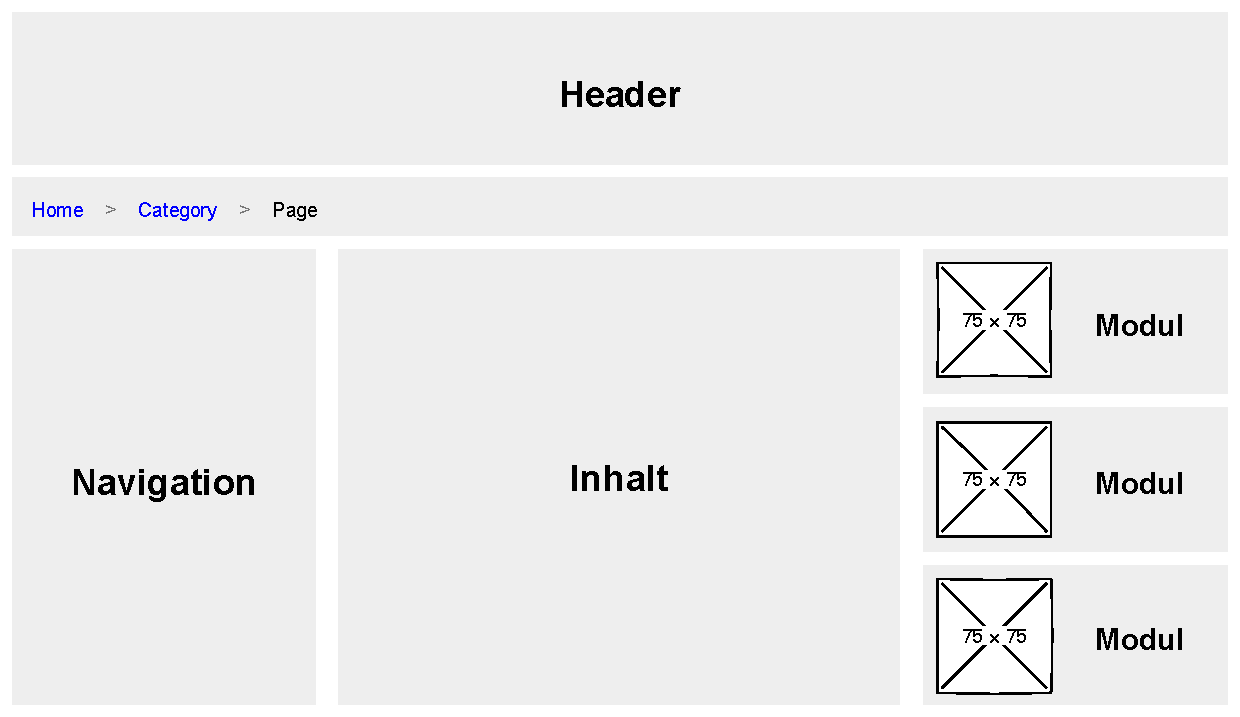
\includegraphics[height=6.5cm]{sketches/grid-example-desktop}%
      \quad
      \includegraphics[height=6.5cm]{sketches/grid-example-mobile}%
    }
  \end{center}
  \caption{Identisches Layout auf großen und kleinen Bildschirmen. Der Navigationsbereich wird für den kleinen Bildschirm nur auf Aufforderung eingeblendet.}
  \label{fig:grid-example}
\end{figure}

Abbildung \ref{fig:grid-example} zeigt das identische Layout aus Zeilen und Spalten in der Darstellung auf unterschiedlich großen Anzeigegeräten. Auf keinem der Geräte werden die beiden obersten Zeilen für den Header und die Pfadangabe weiter in Spalten unterteilt. Diese bestehen technisch gesehen also aus einer einzigen, sehr breiten Spalte.

Die dritte Zeile enthält drei Spalten (Navigation, Inhalt und eine Leiste für Module), wobei diese letzte Modulspalte wiederum mehrere Zeilen enthält. In der mobilen Ansicht wird die Navigationsleiste möglicherweise dynamisch verborgen und kann mit dem Dreieck im Header angezeigt werden. Die Module wandern in dieser Ansicht unter den Inhalt.

\subsubsection{\texttt{HTML}-Bedienelemente}

Grundsätzlich lassen sich alle Bedienelemente anhand der Struktur von Ein- und Ausgaben unterscheiden (Abbildung \ref{fig:ui-element-concept}). Die Unterscheidung, ob eine Ein- bzw. Ausgabe exakt einen Wert oder alternativ mehrere (oder keinen) Wert erwartet bzw. liefert ist für die Oberfläche von zentraler Bedeutung. Die Kapitel \ref{sec:design-ui-bind-output} \nameref{sec:design-ui-bind-output} und \ref{sec:design-ui-bind-input} \nameref{sec:design-ui-bind-input} erläutern diese Unterscheidung noch einmal ausführlich.

\begin{figure}[p]
  \centering \begin{tikzpicture}
  \tikzset{square matrix/.style={
      column sep=-\pgflinewidth, row sep=-\pgflinewidth,
      nodes={
        minimum height=#1,
        anchor=center,
        text width=#1,
        align=center,
        inner sep=6pt
      },
    },
    square matrix/.default=3.50cm
  }


  \matrix[square matrix] (my matrix) at (0,0)
  {
    \node (single)   {Unmittelbare Ausgabe, z.B. in einem Text}; &
    \node (passive)  {Einfaches Eingabelement, z.B. eine Textbox}; \\
    \node (multiple) {Wiederholte Ausgabe, z.B. eine Tabelle}; &
    \node (input)    {Eingabelement mit Mehrfachauswahl}; \\
  };
  \draw [thick,-] (my matrix.east)  |- (my matrix.west);
  \draw [thick,-] (my matrix.south) |- (my matrix.north);

  \node [left=of single, anchor=north, rotate=90] {\textsc{Eine Zeile}};
  \node [left=of multiple, anchor=north, rotate=90] {\textsc{Beliebig}};
  \node [above=of single, anchor=north] {\textsc{Keine Eingabe}};
  \node [above=of passive, anchor=north] {\textsc{Eingabe}};
\end{tikzpicture}



%%% Local Variables:
%%% mode: latex
%%% TeX-master: "../thesis"
%%% End:

  \caption{Einordnung von Bedienelementen}
  \label{fig:ui-element-concept}
\end{figure}

Zwar sollen im Regelfall keine komplett statischen Seiten angezeigt werden, trotzdem muss es natürlich eine Möglichkeit geben statische Texte ohne Bindung an irgendwelche Abfragen zur Anzeige zu bringen. Die hier vorgestellten Bedienelemente funktionieren auch ohne jede Datenquelle, erlauben aber auch die Einbettung von Liquid-Objekten in den Text.

\begin{description}
\item[Überschriften] \hfill \\
  \texttt{HTML} sieht die Verwendung von Überschriften in sechs Hierarchiebenen vor und stellt dafür distinkte Elemente zur Verfügung (\texttt{<h1>} bis \texttt{<h6>}). Dieser Umstand soll nicht unmittelbar abgebildet werden. Stattdessen gibt es ein allgemeines Bedienelement ``Überschrift'', zu dem sich dann eine Ebene angeben lässt.
\item[Absätze] \hfill \\
  Blöcke von zusammenhängendem Text werden als Absatz ausgezeichnet, das entsprechende \texttt{HTML}-Äquivalent ist das \texttt{<p>}-Element.
\item[Listen] \hfill \\
  Strukturiert zusammenhängende Daten werden als sortierte oder unsortierte Liste (\texttt{<ol>} bzw. \texttt{<ul>} in \texttt{HTML}) gruppiert. Wie schon bei den Überschriften soll an dieser Stelle nur ein Bedienelement "`Liste"' zur Verfügung gestellt werden, dass dafür über eine Eigenschaft ``Nummerierung'' verfügt.
\item[Bilder] \hfill \\
  Zwar technisch betrachtet ein eher simples Unterfangen, für Schüler erfahrungsgemäß aber motivierend, ist die Einbindung von Bildern. Diese entsprechen einem \texttt{HTML} \texttt{<img>}-Element, für welches das \texttt{src}-Attribut gesetzt werden muss.
\end{description}

\subsubsection{Komplexe Bedienelemente}
\label{sec:complex-ui-elements}

Viele im Desktopbereiche "`typische"' Bedienelemente haben in reinem \texttt{HTML} keine Entsprechung. So gibt es zum Beispiel jenseits der \texttt{alert()} und \texttt{input()} Funktionen keine standarisierte Möglichkeit modale Dialoge anzuzeigen. Stattdessen existieren je nach Einsatzzweck eine Vielzahl von Bibliotheken. So genannte "`Lightboxen"' kommen zum Einsatz um Bilder nach einem Klick großformatig anzuzeigen, ohne dafür die aktuelle Seite zu verlassen. Und so ziemlich jedes größere \texttt{HTML}-Framework bietet Möglichkeiten, faktisch beliebige \texttt{HTML}-Strukturen im Vordergrund anzuzeigen.

Trotzdem haben sich viele Endanwender an komplexe Webanwendungen gewöhnt, deren Umsetzung um die Jahrtausendwende im Browser vollkommen undenkbar gewesen wäre. Diese Erwartungshaltung bringt \idename{} in ein Dilemma: Gibt man dieser Erwartungshaltung nach und bietet zahlreiche "`künstliche"' Bedienelemente für Spezialfunktionen an, hat das mit der Vermittlung von \texttt{HTML}-Kenntnissen nur noch am Rande etwas zu tun. Andererseits sollen die Lernenden mit "`praktisch vorzeigbaren Ergebnissen"' motiviert werden.

Dieses Spannungsfeld lässt sich gut anhand eines für \idename{} eigentlich zentralen Bedienelements diskutieren: Der Tabelle. Aus didaktischer Sicht scheint es sinnvoll, den Lernenden dieses Element möglichst frühzeitig vorzustellen. Immerhin wird bei den Abfragen mit tabellarischen Daten gearbeitet, da liegt es nahe diese Daten zunächst auf genau diese Art und Weise zu präsentieren.

Allerdings handelt es sich bei Tabellen um eine der deutlich komplizierteren \texttt{HTML}-Konstrukte. Es besteht typischerweise aus zwei unmittelbaren Kindelementen, nämlich \texttt{<thead>} für die Spaltenüberschriften und \texttt{<tbody>} für die eigentlichen Daten. Für neue Zeilen kommen dann die "`Table Row"'-Elemente \texttt{<tr>} zum Einsatz, Zellen werden in den Überschriften dann in \texttt{<th>}-Knoten ("`Table Head"') und im Rumpf mit \texttt{<td>}-Knoten ("`Table Data"') notiert. Und natürlich muss die Anzahl dieser durch Zellenknoten definierten Spalten über alle \texttt{<tr>}-Elemente hinweg identisch sein. Erfahrungsgemäß bereitet es Anfänger auch immer wieder Probleme, dass die in der Tabelle nebeneinander angezeigten Zellen im \texttt{HTML}-Quelltext typischerweise untereinander notiert werden. Und damit nicht genug: Um wirklich alle Zeilen einer Abfrage anzuzeigen, ist die Verwendung von geschachtelten für Zeilen und Spalten Schleifen notwendig. Listing~\ref{lst:html-table-pure} zeigt exemplarisch, wie der nötige Quelltext ausschauen könnte.

\begin{lstlisting}[language=html,float=h,caption={Code für eine \texttt{HTML}-Tabelle mit Datenanbindung}, label={lst:html-table-pure}]
<table>
  <thead>
    <tr>
      
        <th>{{ name }}</th>
      
    </tr>
  </thead>
  <tbody>
    
      <tr>
        
          <td>{{ row[name] }}</td>
        
      </tr>
    
  </tbody>
</table>
\end{lstlisting}

Mit Liquid bietet sich allerdings auch die Möglichkeit, diesen Code weitestgehend vor den Lernenden zu verstecken. Listing~\ref{lst:html-table-liquid} illustriert wie mit der Verwendung des \texttt{include}-Tags die Einbindung der Tabelle auf die Angabe der darzustellenden Zeilen und Spalten reduziert wird. Dabei handelt es sich natürlich nicht um die exakte Darstellung, wie sie innerhalb eines Drag \& Drop Editors dargestellt werden sollte.

\begin{lstlisting}[language=html,float=h,caption={Code für eine Liquid-Tabelle mit Datenanbindung}, label={lst:html-table-liquid}]

\end{lstlisting}

\todo[inline]{HTML-Webcomponents gehen auch in diese Richtung, lösen aber nicht die Datenanbindung}

\subsubsection{Bindung von Abfragen an die Oberfläche}
\label{sec:design-ui-bind-output}

Ein Großteil der Oberflächenelemente wird also einige Eigenschaften aufweisen, deren Inhalte erst zur Laufzeit dynamisch gebunden werden. Dabei stellt sich die Frage, wie die Struktur der zur Verfügung stehenden Daten eigentlich definiert wird bzw. aussehen soll?

Auf abstrakter Ebene ist die Beantwortung dieser Frage eindeutig: Da das Ergebnis einer \texttt{SQL}-Abfrage grundsätzlich eine Tabellenstruktur mit Zeilen, Spalten und Zellen ist, wird dieses Datenmodell auch für die Oberfläche zugrunde gelegt. Die an die Bedienelemente zu bindenden Daten sind also grundsätzlich tabellarischer Natur.

Um im Falle von mehreren in Frage kommenden Abfragen eine eindeutige Zuordnung vornehmen zu können, müssen Abfragen, deren Ergebnis an die Oberfläche gebunden werden soll, mit einem eindeutigen Namen bezeichnet werden. Dieser Name kann von den Entwicklern frei gewählt werden, sollte aber, analog zu einem Funktionsbezeichner, sinnvoll darüber Auskunft geben was eine Abfrage bewirkt. Der Umgang mit den Zeilen erfordert keine Sonderbehandlung, hier genügt die Angabe eines Zeilenindex. Für die Spalten entfällt glücklicherweise eine ``künstliche'' Benennung, diese werden trivialerweise über ihren Namen entsprechend der \texttt{SELECT}-Komponente angesprochen. Mit diesen drei Werten (Name der Abfrage, Zeilenindex, Spaltenname) lässt sich jede Zelle einer Menge von Abfragen eindeutig identifizieren.

Aus praktischen Gründen sollten Abfragen allerdings bezüglich der Anzahl der erwarteten Zeilen annotiert werden können, konkret unterschieden werden muss dabei zwischen ``exakt eine Zeile'' und ``beliebig viele (auch keine) Zeilen''. Im Falle einer Abfrage mit nur einer Zeile entfällt dann Notwendigkeit einen Zeilenindex anzugeben, dieser bezieht sich trivalerweise immer auf die einzige, zur Verfügung stehende Zeile. Wenn Daten an die Oberflächen gebunden werden entfällt durch diese Abkürzung die permanente Angabe einer redundanten Information.

Listing \ref{lst:sql:person-days} zeigt eine Abfrage die in Listing \ref{lst:html:person-days-index} und \ref{lst:html:person-days} einmal mit und einmal ohne Index gebunden wird. Die Schreibweise ohne Index kommt der Lesbarkeit eindeutig zu gute.

\begin{lstlisting}[language=SQL, caption=Abfrage mit garantiert einer Ergebniszeile,label=lst:sql:person-days]
SELECT name, geburtstag
FROM   person
LIMIT  1;
\end{lstlisting}

\begin{lstlisting}[language=HTML, caption=String-Interpolation mit Indexzugriff, label=lst:html:person-days-index]
<!-- benutzer = Listing (*@\ref{lst:sql:person-days}: \nameref{lst:sql:person-days}@*) -->
<p>Hallo {{ benutzer[0].name }}, du bist am {{ benutzer[0].geburtstag }} geboren.</p>
\end{lstlisting}

\begin{lstlisting}[language=HTML, caption=String-Interpolation mit implizitem Index, label=lst:html:person-days]
<!-- benutzer = Listing (*@\ref{lst:sql:person-days}: \nameref{lst:sql:person-days}@*) -->
<p>Hallo {{ benutzer.name }}, du bist am {{ benutzer.geburtstag }} geboren.</p>
\end{lstlisting}

Diese Annotation muss jedoch vom Entwickler manuell im \texttt{SQL}-Editor gesetzt werden, eine automatische Berechnung wäre für beliebige Abfragen unmöglich\footnote{Viele \texttt{SQL}-Dialekte sind Turing-Vollständig und schon das Halteproblem ist nicht entscheidbar.} und auch für speziell strukturierte Abfragen ist diese Unterscheidung zumindest nicht trivial. Oder um es anders auszudrücken: Die Erweiterung der Entwicklungsumgebung um diese automatische Vorhersage wäre Stoff für eine weitere wissenschaftliche Arbeit, keinesfalls aber Gegenstand dieser Arbeit. Praktischerweise lässt sich eine auftretende Verletzung dieser Annotation aber sehr gut erkennen und daher auch sinnvoll an den Entwickler kommunizieren. Und letzten Endes könnte ein Entwickler die Garantie durch die Einführung einer \texttt{LIMIT 1}-Komponente selber geben, was möglicherweise aber zu überraschendem Verhalten zur Laufzeit führt.

Diese gesonderte Behandlung von bestimmten Tabellendimensionen ist übrigens keine Erfindung dieser Thesis: Auch \texttt{SQL} selbst hebt einige Abfragen mit speziellen Strukturen hervor. Tabellen mit nur einer Zelle können als skalarer Wert eingesetzt werden, bei nur einer Spalte können Abfragen z.B. für \texttt{IN}-Ausdrücke verwendet werden.

Der Umgang mit den Zeilen einer Abfrage ist im Rahmen der Oberfläche ein bisschen komplizierter, da hier technisch gesehen häufig zwei verschiedene Elemente zum Einsatz kommen müssen: Ein Containerelement und ein sich wiederholendes Element. Listing \ref{lst:sql:people-days} und \ref{lst:html:people-days} demonstrieren kurz die zu generierende Liquid-Quelle, von der im Drag \& Drop Editor abstrahiert werden müsste.

\begin{lstlisting}[language=SQL, caption=Abfrage mit beliebig vielen Ergebniszeilen,label=lst:sql:people-days]
SELECT name, geburtstag
FROM   person;
\end{lstlisting}

\begin{lstlisting}[language=HTML, caption=Containerelemente mit Kindern, label=lst:html:people-days]
<!-- alleBenutzer = Listing (*@\ref{lst:sql:people-days}: \nameref{lst:sql:people-days}@*) -->
<ul>
  
    <li>
      {{ benutzer.name }} wurde am {{ benutzer.geburtstag }} geboren.
    </li>
  
</ul>
\end{lstlisting}

\subsubsection{Eingabe von Daten über die Oberfläche}
\label{sec:design-ui-bind-input}

Immer wenn eine Abfrage mit Platzhaltern an eine Seite gebunden wird, ist es notwendig dem Benutzer eine Möglichkeit zu geben diese Platzhalter zu füllen. Im einfachsten Fall kann diese Bindung über einfache \texttt{<input type=text>}-Elemente hergestellt werden. Das ist für viele Arten von Such- und Eingabemasken auch sicherlich ausreichend, führt jedoch zu Problemen bei Beziehungen zwischen Entitäten. In diesem Fall müsste in das Textfeld vom Benutzer ein Primärschlüssel angegeben werden, was ganz sicher kein besonders Benutzerfreundliches Konzept darstellt.

In einem solchen Fall soll es also möglich sein auch Bedienelememente wie Comboboxen zu verwenden, die ihrerseits wieder eine Abfrage zur Anzeige der zur Verfügung stehenden Daten benötigen. Dabei muss klar zwischen zwei benötigten Informationen unterschieden werden. Auf der einen Seite muss das Resultat eines solchen Bedienelements vermutlich einen Primärschlüssel zurückliefern. Auf der anderen Seite erwarten die Benutzer aber die Anzeige von ``intuitiven'' Informationen, anhand derer Sie ihre Auswahl treffen können. Der Primärschlüssel ist typischerweise eine künstliche Spalte, die für den Endanwender keinerlei Informationsgehalt hat. Praktischerweise ist auch diese Unterscheidung in \texttt{HTML} vorgesehen

\begin{lstlisting}[float,language=HTML, caption=Containerelemente mit Kindern, label=lst:html:select-example]
<!-- alleBenutzer = Listing (*@\ref{lst:sql:people-days}: \nameref{lst:sql:people-days}@*) -->
<select>
  
    <option value="{{ benutzer.id }}">
      {{ benutzer.name }}
    </option>
  
</select>
\end{lstlisting}

\subsubsection{Navigation}

Die Navigation auf Webseiten teilt sich zwei unterschiedliche Problemstellungen: Noch vor dem Rendervorgang stellt sich die Frage, zu welcher konkreten Seite eine beliebige \texttt{URL} aufgelöst werden soll. Und während der Generierung einer Seite müssen sich Verweise auf andere Seiten erzeugen lassen können.

Damit für jede relevante URL eindeutig ist, zu welcher Seite sie aufgelöst werden soll, könnte man in \idename{} eine zentrale Routing-Konfiguration hinterlegen. In dieser wird einer Menge von Pfaden, welche möglicherweise auch Platzhaltern für Parameter vorsehen, mit den entsprechenden Zielseiten verknüpft. Solche Pfadangaben könnten für das Blogbeispiel wie in Listing~\ref{lst:central-routing-example} angedeutet repräsentiert werden. Bei dem \texttt{selector} handelt es sich um ein Prädikat, welches im Falle einer positiven Auswertung darauf hinweist, dass die entsprechende \texttt{page} dargestellt werden soll.

\begin{lstlisting}[float=h!,caption={Zentrales Routing für das Blog-Beispiel}, label={lst:central-routing-example}]
[
  { "selector": "/",             "page": "Hauptseite" },
  { "selector": "/beitrag/:id",  "page": "Artikel" },
]
\end{lstlisting}

Dabei bedürfen zwei Details besonderer Beachtung: Parameter in der \texttt{URL} werden mit der  \texttt{:parametername}-Notation eingeführt\footnote{Es handelt sich dabei um die gleiche Notation wie sie von den Bibliotheken Sinatra oder Angular 2 verwendet wird.}. Außerdem handelt es sich um eine Liste von Regeln, die Reihenfolge der Einträge ist folglich von Bedeutung. Wenn ein hypothetischer Eintrag mit dem Selektor \texttt{/beitrag/test} eingeführt werden sollte, muss das auf jeden Fall vor dem Selektor \texttt{/beitrag/:id} geschehen. Andererseits passt der Parameter \texttt{:id} auf das \texttt{URL}-Segment \texttt{test} und maskiert diese Route. Unter dieser Randbedingung lässt sich dann aber die Abbildung $\mathtt{URL} \rightarrow \mathtt{Seite}$ eindeutig berechnen.

In diesem Datenmodell können allerdings Inkonsistenzen entstehen, wenn sich die Anzahl oder Benennung der für eine Seite erforderlichen Parameter verändert. Die Behandlung solcher Fehler erfordert allerdings grundsätzlich die Unterstützung des Entwicklers: Nur er kann entscheiden, ob eine umbenannte Variable auch unter neuem Namen semantisch gleichwertig ist. Es handelt sich also um ein Problem, dem am ehesten durch eine passende Benutzeroberfläche beizukommen ist.

Nachdem nun die zu rendernde Seite bekannt ist, stellt sich folglich die inverse Frage: Wie kann die \texttt{URL} zu einer bestimmten Seite generiert werden? Dabei stellt man zunächst fest, dass der \texttt{HTML}-Standard zwei unterschiedliche Mechanismen zur Navigation vorsieht. Die naheliegendste Variante ist die direkte Generierung eines \texttt{<a>}-Knotens mit dem passenden \texttt{href}-Attribut: Mit der Liquid-Syntax lassen sich beliebige Strings generieren, also auch gültige URLs. Allerdings funktioniert dieser Ansatz nur mit Daten, die auf dem Server während des Rendervorgangs bekannt sind. Benutzereingaben in Formularelementen wie \texttt{<input>} können in diesem Kontext nicht verwendet werden.

Es ist folglich schon aufgrund der Vorgaben des \texttt{HTML}-Standards sinnvoll, die Unterstützung von zwei separaten Mechanismen zur Navigation zu unterstützen: Sofern der Endanwender eigene Eingaben vornehmen soll, kommt ein \texttt{<form>}-Element zum Einsatz. Durch die Nutzung von versteckten Eingabelementen (\texttt{<input type="hidden">} können aber auch serverseitig vorhandene Daten, zum Beispiel aus Abfragen oder \texttt{GET}-Parametern innerhalb von Formularen verwendet werden.

\subsection{Drag \& Drop Editor für Oberflächen}
\label{sec:drag-drop-ui-editor}

Für \idename{} stellt sich bei der Gestaltung des Editors für Oberflächen also eine zentrale Frage: Welches Abstraktionsniveau passt zu der avisierten Zielgruppe? Und wie soll zwischen den Zielen "`Motivation durch praktisch vorzeigbare Ergebnisse"' und der Tatsache, dass \idename{} sich als Lehranwendung für HTML versteht, umgegangen werden? Das Abstraktionsniveau kann dabei im wesentlichen auf zwei voneinander weitestgehend unabhängigen Achsen variiert werden: Die erste Achse "`Vorschau"' erstreckt sich sinngemäß von "`Texteditor"' zu "`WYSIWYG-Editor"'. Je näher der Editor an der textuellen Darstellung ist, desto mehr müssen die Schüler gedanklich ergänzen. Die andere Achse ist die Komplexität der zur Verfügung gestellten Bedienelemente, sie geht von "`Reines \texttt{HTML}"' bis hin zu "`Komplexe Bedienelemente"' und wurde schon in Kapitel \ref{sec:complex-ui-elements}~\nameref{sec:complex-ui-elements} diskutiert.

Diese Suche nach dem richtigen Abstraktionsniveau für den den Seiten-Editor wird sich nicht mit einer definitiven Antwort abschließen lassen. Die Anzahl an möglichen Herangehensweisen ist immens, das zeigt schon die Vielfalt an existierenden und historischen Produkten zur Erstellung von Webseiten oder auch "`normalen"' Programmoberflächen.

\subsubsection{Vor- und Nachteile von WYSIWYG-Editoren}
\label{sec:pro-con-wysiwyg-editor}

Programmiersprachen wie Delphi oder Visual Basic verdanken einen Großteil ihrer initialen Popularität auch ihren Entwicklungsumgebungen mit integrierten WYSIWYG-Editoren. Diese ermöglichten es schon zur Entwicklungszeit eine sehr gute Vorschau auf das endgültige Aussehen. Der zeitaufwändige Kreislauf aus "`Wert im Quelltext verändern $\rightarrow$  kompilieren $\rightarrow$ ausführen $\rightarrow$ zu korrekter Maske navigieren $\rightarrow$ Darstellung überprüfen $\rightarrow$ Wert erneut anpassen"' wird drastisch verkürzt. Dieser Ansatz hat aber auch Grenzen: Ohne Kenntnis der genauen Datenbestände bleibt die Vorschau oftmals unvollständig. Und insbesondere bei sehr dynamische Oberflächen mit vielen optionalen Bestandteilen, welche dann häufig zur Laufzeit ein- oder ausgeblendet werden, im Editor aber stehts sichtbar sind, gleicht die Vorschau innerhalb des WYSIWYG-Editors der Endbenutzeransicht dann doch nur noch sehr beschränkt.

Bei der Entwicklung von Desktopanwendungen ist auch heute noch die Verwendung eines WYSIWYG-Editors sehr verbreitet, allerdings werden die Beschreibungen der Oberflächen häufig in spezielle Textdateien ausgelagert. Diese lassen sich dann sowohl mit einem normalen Texteditor bearbeiten als auch mit spezialisierten Editoren bearbeiten. Moderne Bibliotheken für Benutzerschnittstellen wie JavaFX, Android oder die \textit{Windows Presentation Foundation} (WPF) erlauben mit diesem Ansatz die größtmögliche Flexibilät: Jeder Programmierer kann entscheiden, ob er mit der Beschreibungssprache, dem grafischen Werkzeug oder beiden Herangehensweisen arbeiten möchte.

Auch zur Pflege und Generierung von Webseiten existieren und existierten eine Vielzahl unterschiedlicher WYSIWYG-Editoren wie Microsoft Frontpage, Adobe Dreamweaver,~... Diese spielen als Lösungen für hobbymäßige Webseitenbetreiber mittlerweile eine eher untergeordnete Rolle. Heute gängige Lösungen für den Betrieb eigener Webseiten bieten dem Endanwender als primäre Schnittstelle eine im Web verfügbare administrative Oberfläche. Die meisten quelloffenen Content-Management-Systeme wie Wordpress, Joomla oder Typo3 fallen in diese Kategorie. Diese Oberfläche erlaubt es dabei aber vornehmlich den eigentlichen Inhalt der Seiten zu verändern, weniger das Rahmenwerk außen herum. Professionelle Webentwickler halten sich daher von den WYSIWYG-Web-Editoren und editieren lieber unmittelbar die in \texttt{HTML} (oder Skriptsprachen) notierten Templates.

Ein allgemein "`bester"' Ansatz hat sich bis heute also nicht herausgebildet. Dennoch können die gängigen Ansätze zur Bearbeitung von Oberflächen recht gut anhand eines einzigen Merkmals kategorisiert werden: Wie weit ist die im Editor zu sehende Darstellung von der Darstellung im Browser des Endanwenders entfernt? Diese Frage ist natürlich sehr eng verknüpft mit dem fachlichen Hintergrund der Zielgruppe. Ein als "`Webseitenbaukasten für Jedermann"' beworbenes Produkt wird um eine möglichst originalgetreue Darstellung im Editor bemüht sein, fortgeschrittene Entwickler nutzen dann lieber einen Texteditor mit speziellen Hilfsfunktionen wie Syntaxvervollständigung.

Bei WYSIWYG-Webseiten-Editoren handelt es sich im Normalfall um sehr spezielle Anwendungen, mit denen man allerdings sehr schnell Ergebnisse erzielen kann. Hat man eine von Ihnen verstanden, kann der Umgang mit einem konkurierenden Produkt immer noch in vielen Belangen unterschiedlich ausfallen. \texttt{HTML}-Code schaut hingegen in allen Editoren gleich aus und leidet daher weniger unter einem "`Lock-in-Effekt"'.

Insbesondere bei der Visualisierung von Schleifen und bedingten Ausgaben kommt es beim WYSIWYG-Ansatz systemimmanent zu Problemen. Der darzustellende Datenbestand ist im Falle von \idename{} zwar bekannt, es müssen also immerhin keine künstlichen Daten für die Vorschau fingiert werden. Dennoch muss an irgendeiner Stelle der Vorschau auch ein aktuell inaktiver Zweig einer Bedingung oder der abstrakte Schleifenrumpf mit Variablen dargestellt werden können. Endbenutzer werden hingegen niemals beide Seiten einer \texttt{if/else}-Kombination oder die "`Vorlage"' für alle Schritte eines Schleifendurchlaufes zu Gesicht bekommen. Darüber hinaus gibt es in \texttt{HTML} auch noch einige unsichtbare Knoten wie zum Beispiel \texttt{<form>}, \texttt{<audio>} oder \texttt{<menu>}. Diese bedürfen einer "`künstlichen"' visuellen Repräsentation, damit sie bearbeitet werden können. Die WYSIWYG-Darstellung kann also prinzipiell nicht exakt wie beim Endanwender aussehen, sondern muss noch modifiziert werden.

Darüber hinaus bereitet auch das responsive Design der Vorschau Probleme: Es gibt schließlich nicht nur eine Art und Weise die Seite darzustellen, sondern mehrere. Zwischen diesen muss dabei zumindest umgeschaltet werden können.

Ein praktisches Problem bei der Implementierung von WYSIWYG-Editoren ist deren technische Komplexität. Grundsätzlich kann der Code zur Erzeugung der Darstellung für Endanwender nicht 1 zu 1 für die editierbare Darstellung im Editor übernommen werden. Jedes Bedienelement muss im Endeffekt also doppelt implementiert werden\footnote{Im Falle von \idename{} ist das schon aufgrund der unterschiedlichen technischen Grundlagen für Server und Client notwendig (siehe Kapitel \ref{sec:implementation-client-server}~\nameref{sec:implementation-client-server}). Allerdings wird auch in Frameworks mit nur einer Codebasis, zum Beispiel in der .net-Bibliothek WPF, im Code von Bedienelementen explizit zwischen "`Designtime"' und "`Runtime"' unterschieden.}. Bei einer textuellen Repräsentation von \texttt{HTML}-Dokumenten im Editor kann die Darstellung allerdings ausgesprochen gut generalisiert werden. Schließlich handelt es sich im Kern um eine Baum-Darstellung mit einer sehr festen Struktur aus \texttt{XML}-Knoten mit Attributen.

Für einen WYSIWYG-Editor sind hingegen vielfältige Bearbeitungsmöglichkeiten erforderlich. Bilder bedürfen anderer Handgriffe als zum Beispiel Tabellen, Knöpfe oder Links. Um das System für die Entwickler der Entwicklungsumgebung wartbar und für die Lernenden verständlich zu halten, darf an dieser Stelle allerdings auch nicht blind eine spezielle Editorkomponente für jedes Bedienelement entwickelt werden. Es gilt vielmehr die möglichen Gemeinsamkeiten herauszuarbeiten und soweit wie möglich zu generalisieren. Ein dafür zu erstellendes Konzept wäre dabei sowohl technisch als auch fachlich kompliziert..

\subsubsection{Mögliche Ansätze}

Für \idename{} werden daher die folgenden Ansätze auf dem beschriebenen Koordinatensystem eingeordnet und deren individuelle Vor- und Nachteile diskutiert. Drag \& Drop als vornehmliches Bedienparadigma ist dabei für alle Varianten gesetzt, sofern die Beschreibung dies nicht explizit abspricht.

\begin{description}
\item[Vordefinierte Seiten für standarisierte Einsatzzwecke] \hfill \\
  Gedacht für Entwickler, die mit \idename{} einfach nur eine generische Oberfläche für einen Datenbestand erzeugen möchten. Das Layout und die verfügbaren Bedienelemente sind dabei vordefiniert, es können lediglich an vorgesehenen Stellen Abfragen eingebunden, konstante Texte hinterlegt oder ähnliche Parametrisierungen erfolgen. Prinzipiell wäre es auch denkbar, diese Angaben in einer sehr nüchternen, tabellarischen Darstellung vorzunehmen, sinnvoller erscheint im Hinblick auf den Einsatzzweck jedoch eine umfangreiche Vorschau.

  Die wesentliche Herausforderung bei diesem Ansatz ist die Bereitstellung von Vorlagen, welche weder zuviele noch zu wenige an Konfigurationsmöglichkeiten bieten. Ist die Vorlage zu flexibel besteht die Gefahr, dass sie für den Entwickler undurchschaubar wird. Auf der anderen Seite sind zu eingeschränkte Vorlagen aber Gift für kreative Experimente: Wenn die Antwort auf fast jede Idee der Lernenden "`das geht damit nicht"' wäre, kommt vermutlich schnell Frust auf.

  Technisch gesehen ließe sich dieser Ansatz als eine Seite mit einem einzigen, sehr komplexen Bedienelement abbilden.

\item[WYSIWYG Editor für \texttt{HTML}- und Liquid-Blöcke] \hfill \\
  Dieses Vorgehen ähnelt dem Vorgehen von Programmen wie Frontpage oder Dreamweaver. Dem Entwickler wird kein Quelltext präsentiert, sondern eine annotierte Fassung der Vorschau mit all den im vorigen Kapitel beschriebenen Problemen bezüglich der Visualisierung von Schleifen, Verzweigungen und unsichtbaren Elementen.
  
\item[WYSIWYG Layout, \texttt{HTML}- und Liquid-Blöcke] \hfill \\
  Dieser Ansatz kommt dem Entwickler ein Stück weit entgegen, wenn es um die Gestaltung des grundlegenden Layouts, also die Aufteilung in Zeilen und Spalten, geht. 
  
\item[Ausschließlich \texttt{HTML}- und Liquid-Blöcke] \hfill \\
  
\item[Ausschließlich Quelltext] \hfill \\
  
\end{description}

\subsubsection{Grundsätzlicher Aufbau}
\label{sec:design-ui-editor}

\unsure[inline]{Ich bin noch absolut unentschlossen, wie bzw. wo ich die weiteren Eigenschaften von komplexen Eigenschaften unterbringen soll. Die ``klassische'' Variante aller aktuellen Entwicklungsumgebungen ist eine weitere Seitenleiste, die hätte dann in diesem Fall dann allerdings drei Tabs. Daher überlege ich alternativ möglichst viele Informationen unmittelbar im Designbereich unterzubringen. Wenn man dann ein Bedienelement anklickt klappt sich darunter (oder sonstwo) ein Bereich auf, in dem die weiteren Einstellungen vorgenommen werden können.}

Abbildung \ref{fig:ui-editor-sketch-first} zeigt einen möglichen grundsätzlichen Aufbau der Oberfläche aus einem zentralen Designbereich und einer Seitenleiste. Die Verbindungen zwischen den Bedienelementen und den Daten aus der Seitenleiste verdeutlichen zu Illustrationszwecken deren Zusammenhang. In der endgültigen Fassung des Editors soll der Zusammenhang nicht durch Linien dargestellt werden, sondern durch einen Hervorhebungseffekt wenn einer der beiden Seiten aktuell ausgewählt ist.

\unsure[inline]{Eigentlich würde ich gerne auf Tabs in der Seitenleiste verzichten, die Daten könnte man ja auch innerhalb des Designbereiches darstellen. Diesen Weg der Platzierung von nicht sichtbaren Elementen hat auch schon die Delphi IDE betreten und so dramatisch schlimm fand ich das nicht.}

\begin{figure}[h]
  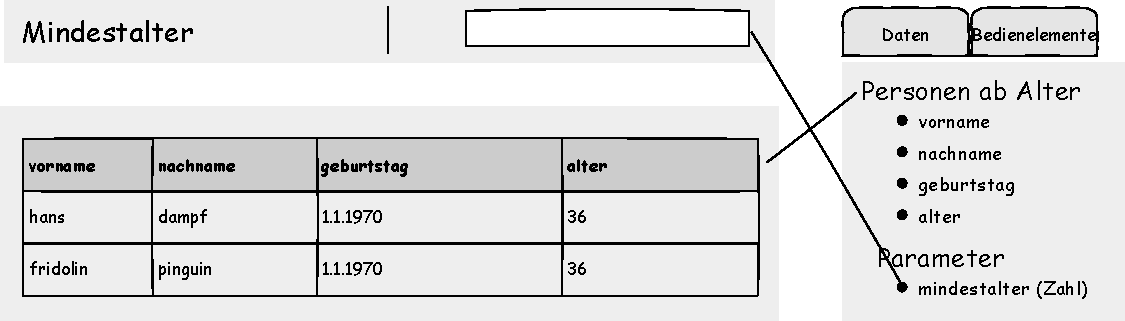
\includegraphics[width=\textwidth]{sketches/ui-sketch-first}
  \caption{Skizze des Oberflächeneditors mit Tabs}
  \label{fig:ui-editor-sketch-first}
\end{figure}

Wenn der Benutzer auf den Tab für die Bedienelemente wechselt, bekommt er eine Übersicht aller verfügbaren Bedienelemente. Diese können dann per Drag \& Drop auf dem Designbereich platziert werden. Einige Bedienelemente verfügen über komplexere Eigenschaften, diese werden dann separat dargestellt.

Um Eigenschaften von Bedienelementen auch ohne spezielle Komponenten editieren zu können, wird in der Seitenleiste ein Editor für Eigenschaften bereitgestellt. Diese Vorgehensweise orientiert sich an den Oberflächen praktisch aller Entwicklungsumgebungen und ermöglicht eine universelle Bearbeitungsmöglichkeit unabhängig von der Repräsentation im eigentlichen Editorbereich. Sowohl ein WYSIWYG- als auch ein "`Block"'-Editor können also, bewusst oder als "`Fallback"', auf identische generische Bearbeitungsmethoden für Bedienelemente zurückgreifen.

\subsubsection{Umgang mit Parametern}

%%% Local Variables:
%%% mode: latex
%%% TeX-master: "thesis"
%%% End:
